%!TEX TS-program = xelatex

\documentclass[a4paper,12pt, landscape]{article}

\usepackage[english,russian]{babel}   %% загружает пакет многоязыковой вёрстки
\usepackage{fontspec}      %% подготавливает загрузку шрифтов Open Type, True Type и др.
\defaultfontfeatures{Ligatures={TeX},Renderer=Basic}  %% свойства шрифтов по умолчанию
\setmainfont[Ligatures={TeX,Historic},
SmallCapsFont={Brill},
SmallCapsFeatures={Letters=SmallCaps}]{Brill} %% задаёт основной шрифт документа
\setsansfont{Brill}                    %% задаёт шрифт без засечек
\setmonofont{Noto Sans Ethiopic}
\usepackage{indentfirst}

%%% Дополнительная работа с математикой
\usepackage{amsmath,amsfonts,amssymb,amsthm,mathtools} % AMS
\usepackage{icomma} % "Умная" запятая: $0,2$ --- число, $0, 2$ --- перечисление

%%% Работа с картинками
\usepackage{wrapfig} % Обтекание рисунков текстом
\usepackage{subcaption}
\usepackage{rotating}
\usepackage{fixltx2e}
\usepackage{hhline}
\usepackage{lscape}
\usepackage[usenames,dvipsnames,svgnames,table,rgb]{xcolor}%пакет для использования цветов 

\usepackage{enumitem}
\setlist{nolistsep, leftmargin=5mm}

%%% Работа с таблицами
\usepackage{array,tabularx,tabulary,booktabs} % Дополнительная работа с таблицами
\usepackage{longtable}  % Длинные таблицы
\usepackage{multirow} % Слияние строк в таблице

\usepackage{multicol} % Несколько колонок

%%% Страница
\usepackage{extsizes} % Возможность сделать 14-й шрифт
\usepackage[twocolumn]{geometry} % Простой способ задавать поля
	\geometry{top=12mm}
	\geometry{bottom=13mm}
	\geometry{left=13mm}
	\geometry{right=9mm}

%\usepackage{fancyhdr} % Колонтитулы
% 	\pagestyle{fancy}
 	%\renewcommand{\headrulewidth}{0pt}  % Толщина линейки, отчеркивающей верхний колонтитул
% 	\lfoot{Нижний левый}
% 	\rfoot{Нижний правый}
% 	\rhead{Верхний правый}
% 	\chead{Верхний в центре}
% 	\lhead{Верхний левый}
%	\cfoot{Нижний в центре} % По умолчанию здесь номер страницы

\usepackage{setspace} % Интерлиньяж
%\onehalfspacing % Интерлиньяж 1.5
%\doublespacing % Интерлиньяж 2
\singlespacing % Интерлиньяж 1

\usepackage{lastpage} % Узнать, сколько всего страниц в документе.
\usepackage{soul} % Модификаторы начертания
\usepackage{bbding}
\usepackage{hyperref}
\usepackage[usenames,dvipsnames,svgnames,table,rgb]{xcolor}
\hypersetup{				% Гиперссылки
    colorlinks=true,       	% false: ссылки в рамках; true: цветные ссылки
    linkcolor=black,          % внутренние ссылки
    citecolor=black,        % на библиографию
    filecolor=black,      % на файлы
    urlcolor=ForestGreen          % на URL
}

\usepackage{environ}
\makeatletter
\newsavebox{\measure@tikzpicture}
\NewEnviron{scaletikzpicturetowidth}[1]{%
	\def\tikz@width{#1}%
	\def\tikzscale{1}\begin{lrbox}{\measure@tikzpicture}%
		\BODY
	\end{lrbox}%
	\pgfmathparse{#1/\wd\measure@tikzpicture}%
	\edef\tikzscale{\pgfmathresult}%
	\BODY
}
\makeatother

\usepackage{pgfplots}
\usepackage{pgfplotstable}
\usepackage{verbatim}

\usepackage{attachfile2}
 \attachfilesetup{appearance=true,
color=0 0 0
 }

%%% Лингвистические пакеты
%\usepackage{savetrees} % пакет, который экономит место
\usepackage{forest} % для рисования деревьев
\usepackage{vowel} % для рисования трапеций гласных
\usepackage{natbib}
\bibpunct[: ]{[}{]}{;}{a}{}{,}
\usepackage[nogroupskip,nopostdot, nonumberlist]{glossaries}
%\usepackage{glossary-mcols} 
%\setglossarystyle{mcolindex}
\usepackage{philex} % пакет для примеров
\addto\captionsrussian{% Replace "english" with the language you use
\renewcommand{\refname}{}
\renewcommand{\glossaryname}{Список глосс}
}
\newcommand{\mytem}{\item[$\circ$]}

\usepackage{todonotes}
\newcounter{mycomment}
\newcommand{\mycom}[1]{
\refstepcounter{mycomment}%
{%
\setstretch{0.7}% spacing
\todo[color=blue!20!white, inline]{%
\textbf{ГМ\themycomment:}~{\footnotesize #1}}%
}}
\renewcommand{\thesection}{\arabic{section}.}
\renewcommand{\thesubsection}{\arabic{section}.\arabic{subsection}}
\setlength{\columnsep}{1.6cm}

\usepackage{sectsty}
\sectionfont{\normalsize}
\subsectionfont{\normalsize}
\usepackage{titlesec}
\titlespacing*{\section}
{0pt}{2ex plus 0ex minus .2ex}{0ex plus .2ex}
\titlespacing*{\subsection}
{0pt}{2ex plus 0ex minus .2ex}{0ex plus .2ex}
\newlength{\bibitemsep}\setlength{\bibitemsep}{.2\baselineskip plus .05\baselineskip minus .05\baselineskip}
\newlength{\bibparskip}\setlength{\bibparskip}{0pt}
\let\oldthebibliography\thebibliography
\renewcommand\thebibliography[1]{%
	\oldthebibliography{#1}%
	\setlength{\parskip}{\bibitemsep}%
	\setlength{\itemsep}{\bibparskip}%
}
\usepackage{alltt}
\begin{document}
\begin{flushright}
	{\footnotesize Г. Мороз, а. Ходзь, Республика Адыгея}
\end{flushright}
\begin{center}{\Large Скорость речи кубанского диалекта кабардино-черкесского языка\footnote{Автор выражает благодарности:
\begin{itemize}
\mytem Ване Левину, Саше Мартыновой, Лене Пасальской и Соне Сиговой за помощь в придумывании историй;
\mytem Тане Руссите за рисунки;
\mytem Информантам Аминат Мухарбиевне Бижоевой, Зурьят Тутовне Нагоевой, Ирме Аскарбиевне Афашаговой, Жанне Магомедовне Мамижевой, Асе Аскарбиевне ??, Анзору Шхамбиевичу Бегеретову, Майе Джабраиловне Терчуковой,  Ахмеду Абрековичу Бегеретову и Фатиме ?? ?? за участие в эксперименте;
\mytem Сиговой Соне за помощь в разборе текстов;
\mytem Юре Ландеру за помощь в глоссировании текстов;
\mytem ... за комментарии.
\end{itemize}}}
\end{center}
{\noindent\footnotesize последняя версия: \textbf{\href{https://goo.gl/hxov2y}{https://goo.gl/hxov2y}}}
\tableofcontents
\vfill
\pagebreak
\section{Введение}
\subsection{Обзор литературы}
\noindent Судя по всему, о скорости речи говорили еще в начале XX века, но первые квантитативные исследования, начались, видимо, с работ \citep{goldman54} и \citep{goldman56}; и с самых ранних работ данная тема затрагивала еще и некоторые аспекты психиатрии. Данная тема тесно соприкасается с разницей ударных и безударных слогов, а также ритмической структуры слова, фразы и т. п.
\par В исследовании \citep{goldman54} исследовались по три интервью от пяти пациентов, собранных тремя психиатрами. В качестве характеристики скорости речи используется количество слов в минуту и стандартное отклонение полученной величины. В следующей работе \citep{goldman56} автор был более эксплицитен и ввел некоторые важные понятия:
\begin{itemize}
\mytem \textbf{общая скорость речи} (total or overall Speech Rate), которая высчитывается по формуле ${ns}/t$, где ${ns}$ --- это количество слогов во всех высказываниях, a $t$ --- общая длительность всех высказываний.
\mytem \textbf{скорость артикуляции} или \textbf{абсолютная скорость речи} (Articulation Rate), которая высчитывается по формуле $ns/ts$, где $ns$ --- это количество слогов во всех высказываниях, a $ts$ --- время чистого говорения.
\mytem \textbf{пропорциональная длительность пауз}, которая высчитывается по формуле $tp/t$, где $tp$ --- это длительность пауз во всех высказываниях, a $t$ --- общая длительность всех высказываний.
\mytem \textbf{скорость дыхания} (Respiration Rate), которая по формуле $ni/t$, где ${ni}$ --- это количество вдохов во всех высказываниях, a $t$ --- общая длительность всех высказываний.
\end{itemize}
\par Среди результатов работы \citep{goldman56} отмечается отрицательная корреляция между общей скоростью речи и пропорциональной длительностью пауз, т. е. чем длиннее и чем дольше паузы, тем меньше общая скорость речи. В исследовании также подчеркивается, что скорость дыхания, измеряемая в процессе речи, отличается от действительной скорости дыхания, так как в ней происходит выдыхательная задержка, вызванная процессом речепроизводства.
\par Работа \citep{fonagy60} начинается с перечислении идей разных фонетистов о разной скорости, с которой произносятся слова разной длины: длинные слова произносятся быстрее, короткие слова --- медленнее. Потом автор переходит к единицам, которые он называет \textit{ритмическим периодом} (rhythmical period). Автор показывает, что связь между \textbf{средней длиной звука в ритмической единице} экспоненциально зависит от количества звуков в данной единице. В данной работе тоже анализировалось дыхание, а именно информанты читали текст, а исследователь смотрел, где происходит вдох. Длинна ритмической единицы, а следовательно, как считает автор, и скорость, зависят от речевого материала (поэзия, проза, диалог, спортивный комментарий и т. п.), а увеличение скорости в более длинных единицах не связано с дыхательными циклами. 
\par В работе \citep{osser64}  сравнивались скорости речи американских и японских студентов, которая измерялась количеством фонем в минуту. Обнаружилось, что в среднем японские студенты говорили несколько медленнее, однако разница не была статистически значимой. Кроме того, исследователи провели довольно странный эксперимент, в котором они просили респондентов назвать как можно больше слов за одну минуту. Японцы и здесь показали меньший результат, но и в этом эксперименте разница была статистически не значимой. Авторы продолжают делать некоторые выводы относительно, результатов теста Стьюдента, однако в корректности данных выводов можно усомниться.
\par В работе \citep{barik77} анализировались скорость речи (\textbf{общая скорость речи} --- количество слогов в минуту, \textbf{скорость артикуляции} --- количество слогов в минуту без учета пауз и некоторые другие параметры) в разных режимах речи на английском и французском языках:
\begin{itemize}
\mytem спонтанная речь (составленные на основе картинок истории, обсуждения последнего фильма);
\mytem полуспонтанная речь (записи лекции приглашенных лекторов);
\mytem подготовленное устное сообщение 
\mytem подготовленное письменное сообщение (чтение фрагмента статьи)
\end{itemize}
\par Работа \citep{vaane82} проверяла гипотезу, сформулированную ранее, предполагавшая, что речь на незнакомом языке воспринимается как более быстрая, так как паузы, хезитация и т. п. слушающим не воспринимаются как таковые, в результате, слушающий из двух фрагментов спонтанной речи с примерно одинаковой скоростью, фрагмент на незнакомом будет считать более быстрым, чем фрагмент на родном языке. В работе \citep{vaane82} на материале нидерландского, английского, французского, испанского и арабского был проведен психолингвистический эксперимент, показавший, что данная гипотеза не верна.
\par Работа \citep{uhmann92} посвящена восприятию скорости. Кроме стандартных методов вычисления скорости (звуки, слова, слоги / в некоторый момент времени) автор описывает метод, предложенный в работе, в котором предлагается анализировать количество ударных слогов в просодической единице. Кроме того, в работе вместо термина \textit{скорость} использовать термин \textit{плотность}, что связано с перцептивной направленностью работы. В работе также высказывается предположение, что на восприятие скорости речи влияет количество пропущенных слогов, хотя и отмечается, что достаточно часто данный подход будет встречать значительные трудности. Достаточно важным открытием, сделанным в данной работе, является обнаружение, того, что речь воспринимается быстрой, если высокими являются показатели скорости (в терминах автора --- плотности), измеряемые и в слогах, и в ударных слогах. Если хотя бы один из данных является низким, то речь как быстрая не воспринимается.
\par В работах \citep{verhoeven04} и \citep{quene08} анализировался большой корпус интервью нидерландских учителей (160 носителей) из разных регионов Нидерландов и Бельгии. В первой работе основной акцент был сделан на различия между носителями и в результате получилось, что мужчины говорят быстрее, чем женщины\footnote{Все время в данных экспериментах не указывают какого пола был интервьюер, ведь можно допустить, что мужчины быстрее говорят  с мужчинами, а женщины --- с женщинами, а указанный эффект возникает от того, что интервьюер является мужчиной.}, люди старшего возраста говорят быстрее, чем люди младшего возраста, а люди из Фландрии говорят медленнее, чем в остальных регионах. Во второй работе проводился не только анализ вариативности между носителями, но и исследовалась изменение скорости речи в зависимости от размера фразы. В целом, в работе \citep{verhoeven04} используется более сложная статистика, подтвердившая результаты первого исследования, а что касается второй части работы, то она согласуется с результатами  работы \citep{fonagy60}: также получена экспоненциальная зависимость между количеством слогов в слове и длительностью фразы.
\par В работе \citep{hilton11} сравниваются датский, норвежский и шведский, однако акцент в данной работе сделан на редукции сегментов в быстрой речи, которая в разной степени проявлена в данных языках (автор приводит пример сокращения пяти слогов до одного в датском). В результате оказалось, что скорость датской речи несколько больше скорости шведской и норвежской речи, что видимо, и произошло за счет тех масштабных процессов сокращения слогов.
\par Работа \citep{stepanova11}, посвящена исследованию русского языка. Базой для исследования послужили записи проекта "Один речевой день", в рамках которого были записаны 46 информантов разного возраста, социального положения и т. п. В целом результаты совпадают с предыдущими исследователями (например, \citep{verhoeven04} для нидерландского):
\begin{itemize}
\mytem мужчины говорят быстрее женщин (аналогичные результаты были получены для американского английского, китайского и нидерландского)
\mytem чем длиннее просодическая единица, тем быстрее она произносится
\mytem выделена возрастная граница, после которой носители говорят обычно медленнее
\end{itemize}
\subsection{Промежуточные итоги}
\begin{itemize}
\mytem Скорость речи определяют как скорость появления языковых единиц в течении некоторого промежутка времени. В литературе предлагались разные методы измерения скорости речи:
\begin{itemize}
\item количество звуков в промежуток речи или на просодическую единицу
\item количество слогов в промежуток речи или на просодическую единицу
\item количество ударных слогов в промежуток речи или на просодическую единицу
\item количество слов в промежуток речи или на просодическую единицу
\end{itemize}
Последний вариант меньше всего претендует на универсальность, так как длинна слов может варьироваться от языка к языку, да и понятие \textit{слова} достаточно размыто. В связи с этим данное измерение на нашем материале не производилось. Стоит оговорится, что метод подсчета слогов тоже несколько не универсален, так как бывают языки, в которых распространены достаточно сложные слоговые структуры, производство которых в целом занимают чуть больше времени, чем простые слоги CV, которые являются единственным типом слога, например, в гавайском.
\mytem Насколько известно, нет данных свидетельствующих в пользу того, что в адыгских языках есть слоговые согласные, так что мерой для измерения количества слогов в данной работе будет считаться количество гласных.
\mytem Различают несколько параметров, характеризуюшие паузы
\begin{itemize}
\item внутри/снаружи интонационной группы
\item заполненная/незаполненная
\item имеющие дискурсивную роль/вызванные экстралингвистическими причинами
\end{itemize}
Перед исследованием, следует принять решения, относительно того, считаются ли заполненные паузы (например, с "э-э-э") слогом и т. п. проблемы.
\mytem В некоторых работах высказывались предположения о связи дыхания и скорости речи, так что имело бы смысл сравнивать обычное дыхание говорящего и сравнивать его с дыханием во время речепроизводства. Однако для данного исследования понадобился бы пнеумотахограф --- на обычной  аудиозаписи дыхания не слышно (к тому же, возможно, Жанна задержала дыхания, когда мы пробовали записать ее на диктофон).
\mytem Было бы интересно посмотреть будет ли пол и возраст влиять на скорость речи (как в \citep{stepanova11}), но наша выборка нерепрезентативна.
\mytem Важно смотреть не только различия в скорости между носителями, но и зависимость скорости от длинны фразы или другой просодической единицы.
\end{itemize}
\subsection{Вопросы данной работы}
\begin{itemize}
\mytem Какая средняя скорость речи в нарративах? Насколько велика дисперсия данного значения? Как полученная скорость соотносится с результатами полученными для других языков? (between-speaker variation)
\mytem Насколько окажутся скоррелированы разные методы измерения скорости речи?
\mytem Насколько сильно различаются скорости речи в нарративах, рассказанных по картинкам, от скорости чтения текста? Подтверждаются ли наблюдения сделанные на основе других языков?
\mytem Какие характеристики нарративов будут влиять на суждения информантов о скорости речи?
\mytem Как зависит скорость речи от длинны ЭДЕ? (within-speaker differences)
\mytem Существуют ли общие фонологические/фонетические особенности устного дискурса (мы мечтали, конечно, о <<беглой спонтанной речи>>), отличных от результатов элицитации?
\item[{\DejaSans \symbol{"1F63C}}] В принципе данную работу хорошо бы провести и в других аулах, чтобы можно было сравнивать близкородственные языки.
\end{itemize}
\section{Ход эксперимента}
\noindent Эксперимент состоял из нескольких частей. Девять информантов (семеро женщин и двое мужчин) рассказывали истории по картинкам (картинки представлены в разделе \ref{pictures}, а полученные истории в разделе \ref{corpus}), кроме того всем информантам было предложено прочитать прозаический текст (см. раздел \ref{text}) и стихотворный текст (см. раздел \ref{verse}). Таким образом в эксперимент попали тексты трех разных стилей. Рассказы по картинкам были записаны особым образом: информанты сидели по двое, и каждый рассказывал другому свою историю, т. е. каждый информант слышал одну историю, и рассказывал другую.
\par Записанные тексты разбирались в ELAN (v. 4.9.4), потом создавался слой с количеством слогов и экспортировался в файл .TextGrid (файл для аннотации файлов в Praat). Далее в Praat (v. 5.3.16) скриптом (см. раздел \ref{praatscript}) собиралась информация о длительности всех сегментов в отдельный файл .csv, который потом анализировался в R (v. 3.3.1, см. раздел \ref{Rscript}).
\par Так как из 10 информантов, каждый слышал по две истории (одну рассказывал, другую слушал), для перцептивного эксперимента оставшиеся восемь историй были разделены на следующие группы:
\begin{itemize}
\mytem 3 истории были оставлены без изменений
\mytem 2 истории были слегка замедлены (на x\%)
\mytem 2 истории были слегка ускорены (на x\%)
\mytem 1 история была значительно ускорена (на y\%)
\end{itemize}
\section{Результаты}
\subsection{Средние значения скорости речи и чтения}
\noindent В данной работе основным измерением мы будем считать \textbf{абсолютную скорость речи} (Articulation Rate), т. е. учитывается скорость речи внутри ЭДЕ а паузы между ЭДЕ в расчет не берутся. Подсчеты будут вестись в количестве слогов в секунду, а те в свою очередь будут считаться на основании количества гласных.
\begin{figure}[t]
\begin{subfigure}[b]{0.53\textwidth}
        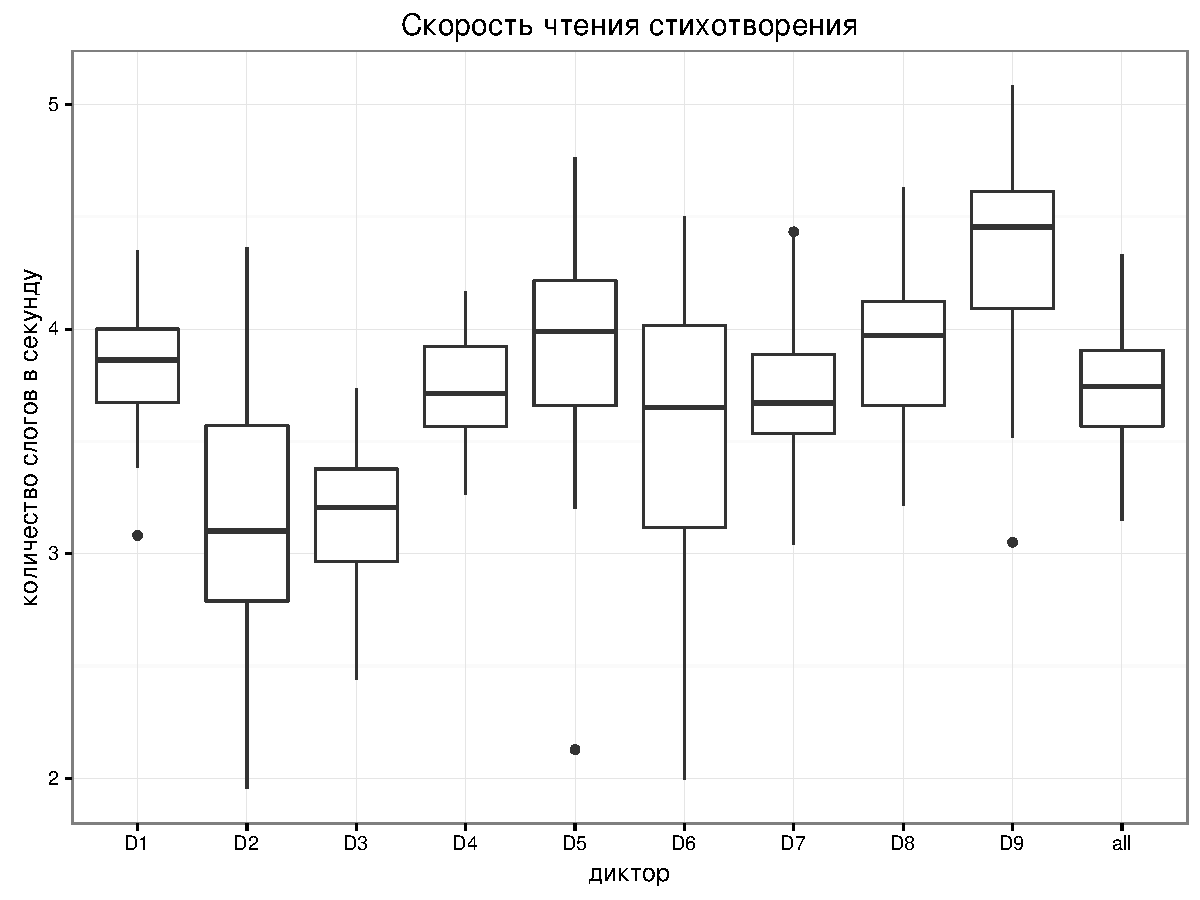
\includegraphics[width=\linewidth]{verseboxplot.pdf}
        \caption{боксплоты полученных значений}
\end{subfigure}
\hfill
\begin{subfigure}[b]{0.45\textwidth}
\small
\begin{tabular}{|l|l|l|l|}
\hline
диктор & средняя скорость & 95\% conf. int. & sd \\ \hline
D1 & 3.852108 & ±0.07830897 & 0.2989850 \\ \hline
D2 & 3.146742 & ±0.20756448 & 0.5603714 \\ \hline
D3 & 3.165385 & ±0.12043343 & 0.3251397 \\ \hline
D4 & 3.744444 & ±0.09374592 & 0.2530902 \\ \hline
D5 & 3.905876 & ±0.19486083 & 0.5260748 \\ \hline
D6 & 3.567189 & ±0.23055344 & 0.6224358 \\ \hline
D7 & 3.728681 & ±0.13946132 & 0.3765102 \\ \hline
D8 & 3.915931 & ±0.13679059 & 0.3692999 \\ \hline
D9 & 4.330937 & ±0.16841999 & 0.4546912 \\ \hline
all & 3.720940 & ±0.06309752 & 0.5386854 \\ \hline
\multicolumn{1}{c}{}&\multicolumn{1}{c}{}&\multicolumn{1}{c}{}&\multicolumn{1}{c}{}\\
\multicolumn{1}{c}{}&\multicolumn{1}{c}{}&\multicolumn{1}{c}{}&\multicolumn{1}{c}{}\\
\end{tabular}
\normalsize
\caption{полученные значения}        
\end{subfigure}
\caption{Скорость чтения стихотворения каждым информантом (D1-D9) и всеми вместе (all)}
\label{verseboxplot}
\end{figure}
\par На рисунке \ref{verseboxplot} представлены результаты измерений скорости чтения стихотворения. Скорость измерялась в количествах слогов в секунду. В целом, полученные результаты отражают умения читать информантов: те информанты, которые плохо читают, часто запинаются или делают паузы посреди строк стихотворения, так что в их чтении есть как много быстрых произнесений, так и много медленных. Такие информанты (D2 и D6) имеют больший разброс усов боксплота (напомню, что ус не может привышать 1.5 межквартильных расстояния), больший разброс доверительного интервала. Стандартное отклонение у таких информантов почти на треть больше, чем у информантов, которые хорошо читают. Средняя скорость чтения стихотворения составила 3.72 слога в секунду c 95\% доверительным интервалом равным 0.06 и стандартным отклонением 0.54 слога в секунду. Надо оговорится, что нельзя утверждать, что те информанты, которые хорошо читают, читают стихи быстрее --- один информант (D3) читал стихи с выражением и медленно. Однако хоть скорость речи у информанта D3 и низкая, но доверительный интервал и стандартное отклонение у него достаточно низкие --- хороший чтец читает более ли менее на одной скорости, в то время как плохой чтец запинается вставляет паузы, таким образом его речь содержит как очень быстрые фрагменты, так и крайне медленные.
\begin{figure}[t]
\begin{subfigure}[b]{0.53\textwidth}
        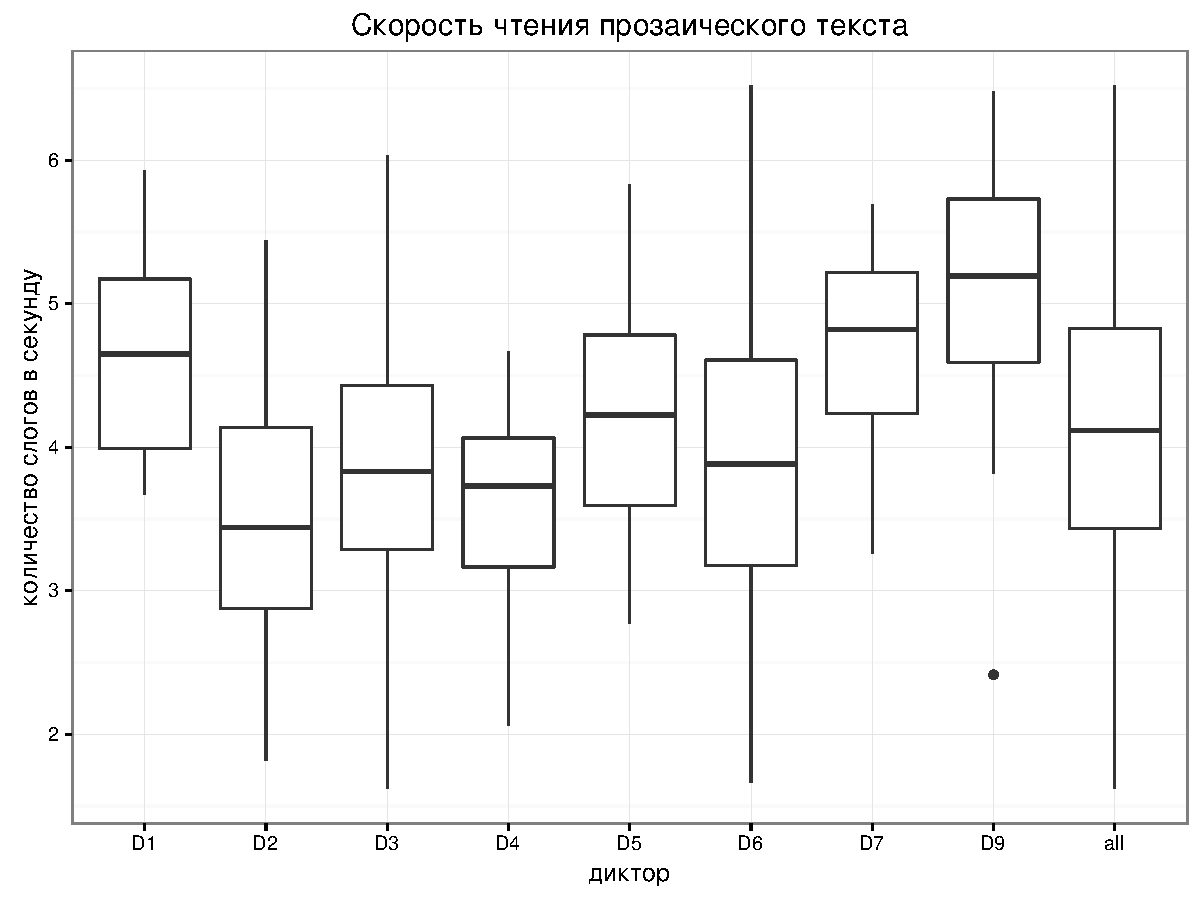
\includegraphics[width=\linewidth]{proseboxplot.pdf}
        \caption{боксплоты полученных значений}
\end{subfigure}
\hfill
\begin{subfigure}[b]{0.45\textwidth}
\small
\begin{tabular}{|l|l|l|l|}
\hline
диктор & средняя скорость & 95\% conf. int. & sd \\ \hline
D1 & 4.632069 & ±0.2490640 & 0.6602932 \\ \hline
D2 & 3.524537 & ±0.3387037 & 0.9305997 \\ \hline
D3 & 3.824807 & ±0.3247948 & 0.8923844 \\ \hline
D4 & 3.601797 & ±0.2324025 & 0.6274278 \\ \hline
D5 & 4.154894 & ±0.3073855 & 0.7841468 \\ \hline
D6 & 3.974244 & ±0.4396417 & 1.1437458 \\ \hline
D7 & 4.733744 & ±0.2994228 & 0.7165394 \\ \hline
D8 &  & ± &  \\ \hline
D9 & 5.008959 & ±0.4027820 & 1.0478538 \\ \hline
all & 4.153892 & ±0.1345448 & 0.9994908 \\ \hline
\multicolumn{1}{c}{}&\multicolumn{1}{c}{}&\multicolumn{1}{c}{}&\multicolumn{1}{c}{}\\
\multicolumn{1}{c}{}&\multicolumn{1}{c}{}&\multicolumn{1}{c}{}&\multicolumn{1}{c}{}\\
\end{tabular}
\normalsize
\caption{полученные значения}        
\end{subfigure}
\caption{Скорость чтения прозаического текста каждым информантом (D1-D9) и всеми вместе (all)}
\label{proseboxplot}
\end{figure}
\par На рисунке (\ref{verseboxplot}) представлены результаты измерений скорости чтения прозаического текста. В целом, все информанты кроме четвертого читали прозаический текст быстрее, чем стихотворный. Скорость в среднем больше на 0.49 слога в секунду (от 0.20 слога в секунду до 1 слога в секунду). Кроме того больше и стандартное отклонение: в среднем на 0.42 слога в секунду (от 0.25 слога в секунду до 0.59 слога в секунду). Средняя скорость чтения стихотворения составила 4.15 слога в секунду c 95\% доверительным интервалом равным 0.13 и стандартным отклонением в 1 слог в секунду.
\subsection{Сравнение разных методов измерения скорости речи}
\subsection{Перцептивный эксперимент}
\subsection{Скорость речи внутри нарратива}
\pagebreak
\section{Фонологические/фонетические особенности}
\subsection{Транскрипционные замечания}
\noindent Достаточно сложным этапом работы является поиск соответствий между аудиозаписью и той транскрипцией, которая получается в результате разбор текста с информантом. Информанты ориентируются на то, что ``должно'' быть сказано, а не на то, как это сказано, поэтому часто оговорки и сокращения при разборе текстов пропускаются. В нашем исследовании, мы наоборот старались в разборе показать фальстарты, паузы, обрывы слов и т. п., ориентируясь на принципы сформулированные в работе \citep{kibrik14}:
\lb{breaks}{\gll  qχʷe-r= ee(1.4) fəzə-m qχʷe-r jə-r-jə-xʷəẑ-a\\
свинья-\textsc{abs} \textsc{hes} женщина-\textsc{obl} свинья-\textsc{abs} \textsc{loc-dat-3sg.erg}-прогнать-\textsc{pst}\\
\trans ‘Свинья= э-э женщина свинью прогнала.’ \hfill D1, 0:20.96--0:26.16\footnote{Рядом с текстами мы будем писать номер диктора, а потом время в формате минуты:секунды.милисекунды. Все тексты приведены в разделе \ref{corpus}.}}
\par В данной записи знаком равно обозначен обрыв слова, ee(1.4) --- это заполненная пауза и в скобках длительность данной паузы (незаполненные паузы обозначаются многоточием). Русские вкрапления в текстах транслитирируются и выделяются жирным курсивом (см., например, (\ref{omission}), (\ref{insertion}) и другие).
\par Достаточно важно различать то, что носители произносят, и то, что носители считают, что произносят. Часто носители при разборе додумывают то, что должно было быть сказано в данный момент, хотя на деле в аудиозаписи часть ожидаемого материала отсутствует. Такие опущения в аудиозаписи в транскрипции текстов мы обозначили квадратными скобками, например:
\lb{omission}{\gll  \textbf{\textit{i}} pŝaf̣ə-re qχʷe-r \underline{\textbf{[qə-]č̣e-[rə-]ɬade-r-jə}} \\
и готовить-\textsc{add} свинья-\textsc{abs} \underline{\textsc{dir-loc-?-}бежать-\textsc{cvb-add}} \\
\trans ‘И пока она готовила, свинья подбежала…’ \hfill D9, 0:06.32--0:14.36}
То есть, в примере (\ref{omission}) диктор произнес \textbf{č̣eɬaderjə}, однако несколько информантов (в том числе диктор) подтвердили, что имелось в виду \textbf{qəč̣erəɬaderjə}. При этом информанты даже соглашаются, что произнесено не совсем то, однако все равно настаивают  на том, что сказано именно \textbf{qəč̣erəɬaderjə}.
\par Бывают обратные случаи, когда информант произнес какой-то лишний звук, которого не должно в данной морфеме, такие оговорки мы обозначили угловыми скобками, например:
\lb{insertion}{\gll \textbf{\textit{koroč'e}} \textbf{\textit{pauk}}ə-m-re \textbf{\textit{djatel}}ə-m-re ze-\textbf{\underline{<wə>}}χʷen-xe-r-jə \\
короче паук-\textsc{obl-add} дятел-\textsc{obl-add} \textsc{rec}-ругаться-\textsc{pl-cvb-add}\\
\trans `Короче, паук и дятел поссорились и …' \hfill D8, 0:19.70-0:22.59}
То есть, в примере (\ref{insertion}) диктор произнес \textbf{zewəχʷenxerjə}, однако иинформанты признают верным лишь вариант \textbf{zeχʷenxerjə}.
\par Полученные нарративы были разделены на \textbf{элементарные дискурсивные единицы} (далее \textbf{ЭДЕ}) --- минимальные единицы, на которые делится дискурс (подробнее см. \cite[55--102]{kibrik14} и приведенную там литературу). В сборнике \cite[60]{kibrik14} предлагается выделять ЭДЕ на основе:
\begin{itemize}
\mytem тонального паттерна (возвращение к базовому F0 уровню в начале, падение F0 к концу)
\mytem наличия единственного акцентного центра
\mytem темпового паттерна (ускорение в начале ЭДЕ, замедление к концу)
\mytem паттерна интенсивности (высокая громкость в начале, затихание в конце)
\mytem пограничные паузы
\end{itemize}
В нашей работе при выделении ЭДЕ мы будем стараться ориентироваться на интонацию, наличие акцентного центра, синтаксического единства и пограничные паузы.
\vfill 
\pagebreak
\footnotesize
\noindent Список сокращений и глосс
\begin{multicols}{2}
\noindent …(1.3) --- незаполненная пауза и ее длительность\\
$\left[\mbox{rə-}\right]$ --- значимый фрагмент, отсутствующий в аудиозаписи\\
<wə> --- лишний фрагмент, присутствующий в аудиозаписи\\
 = --- обрыв слова или фальстарт\\
ee(1.3) --- незаполненная пауза и ее длительность\\
\textbf{\textit{koroč'e}} --- русские заимствования транслитерируются и выделяются жирным курсивом\\
\end{multicols}
\bibliographystyle{chicago}
\bibliography{bibliography}
\normalsize
\section{Приложения}
\subsection{Приложение 1: изображения Тани Русситы} \label{pictures}
\noindent 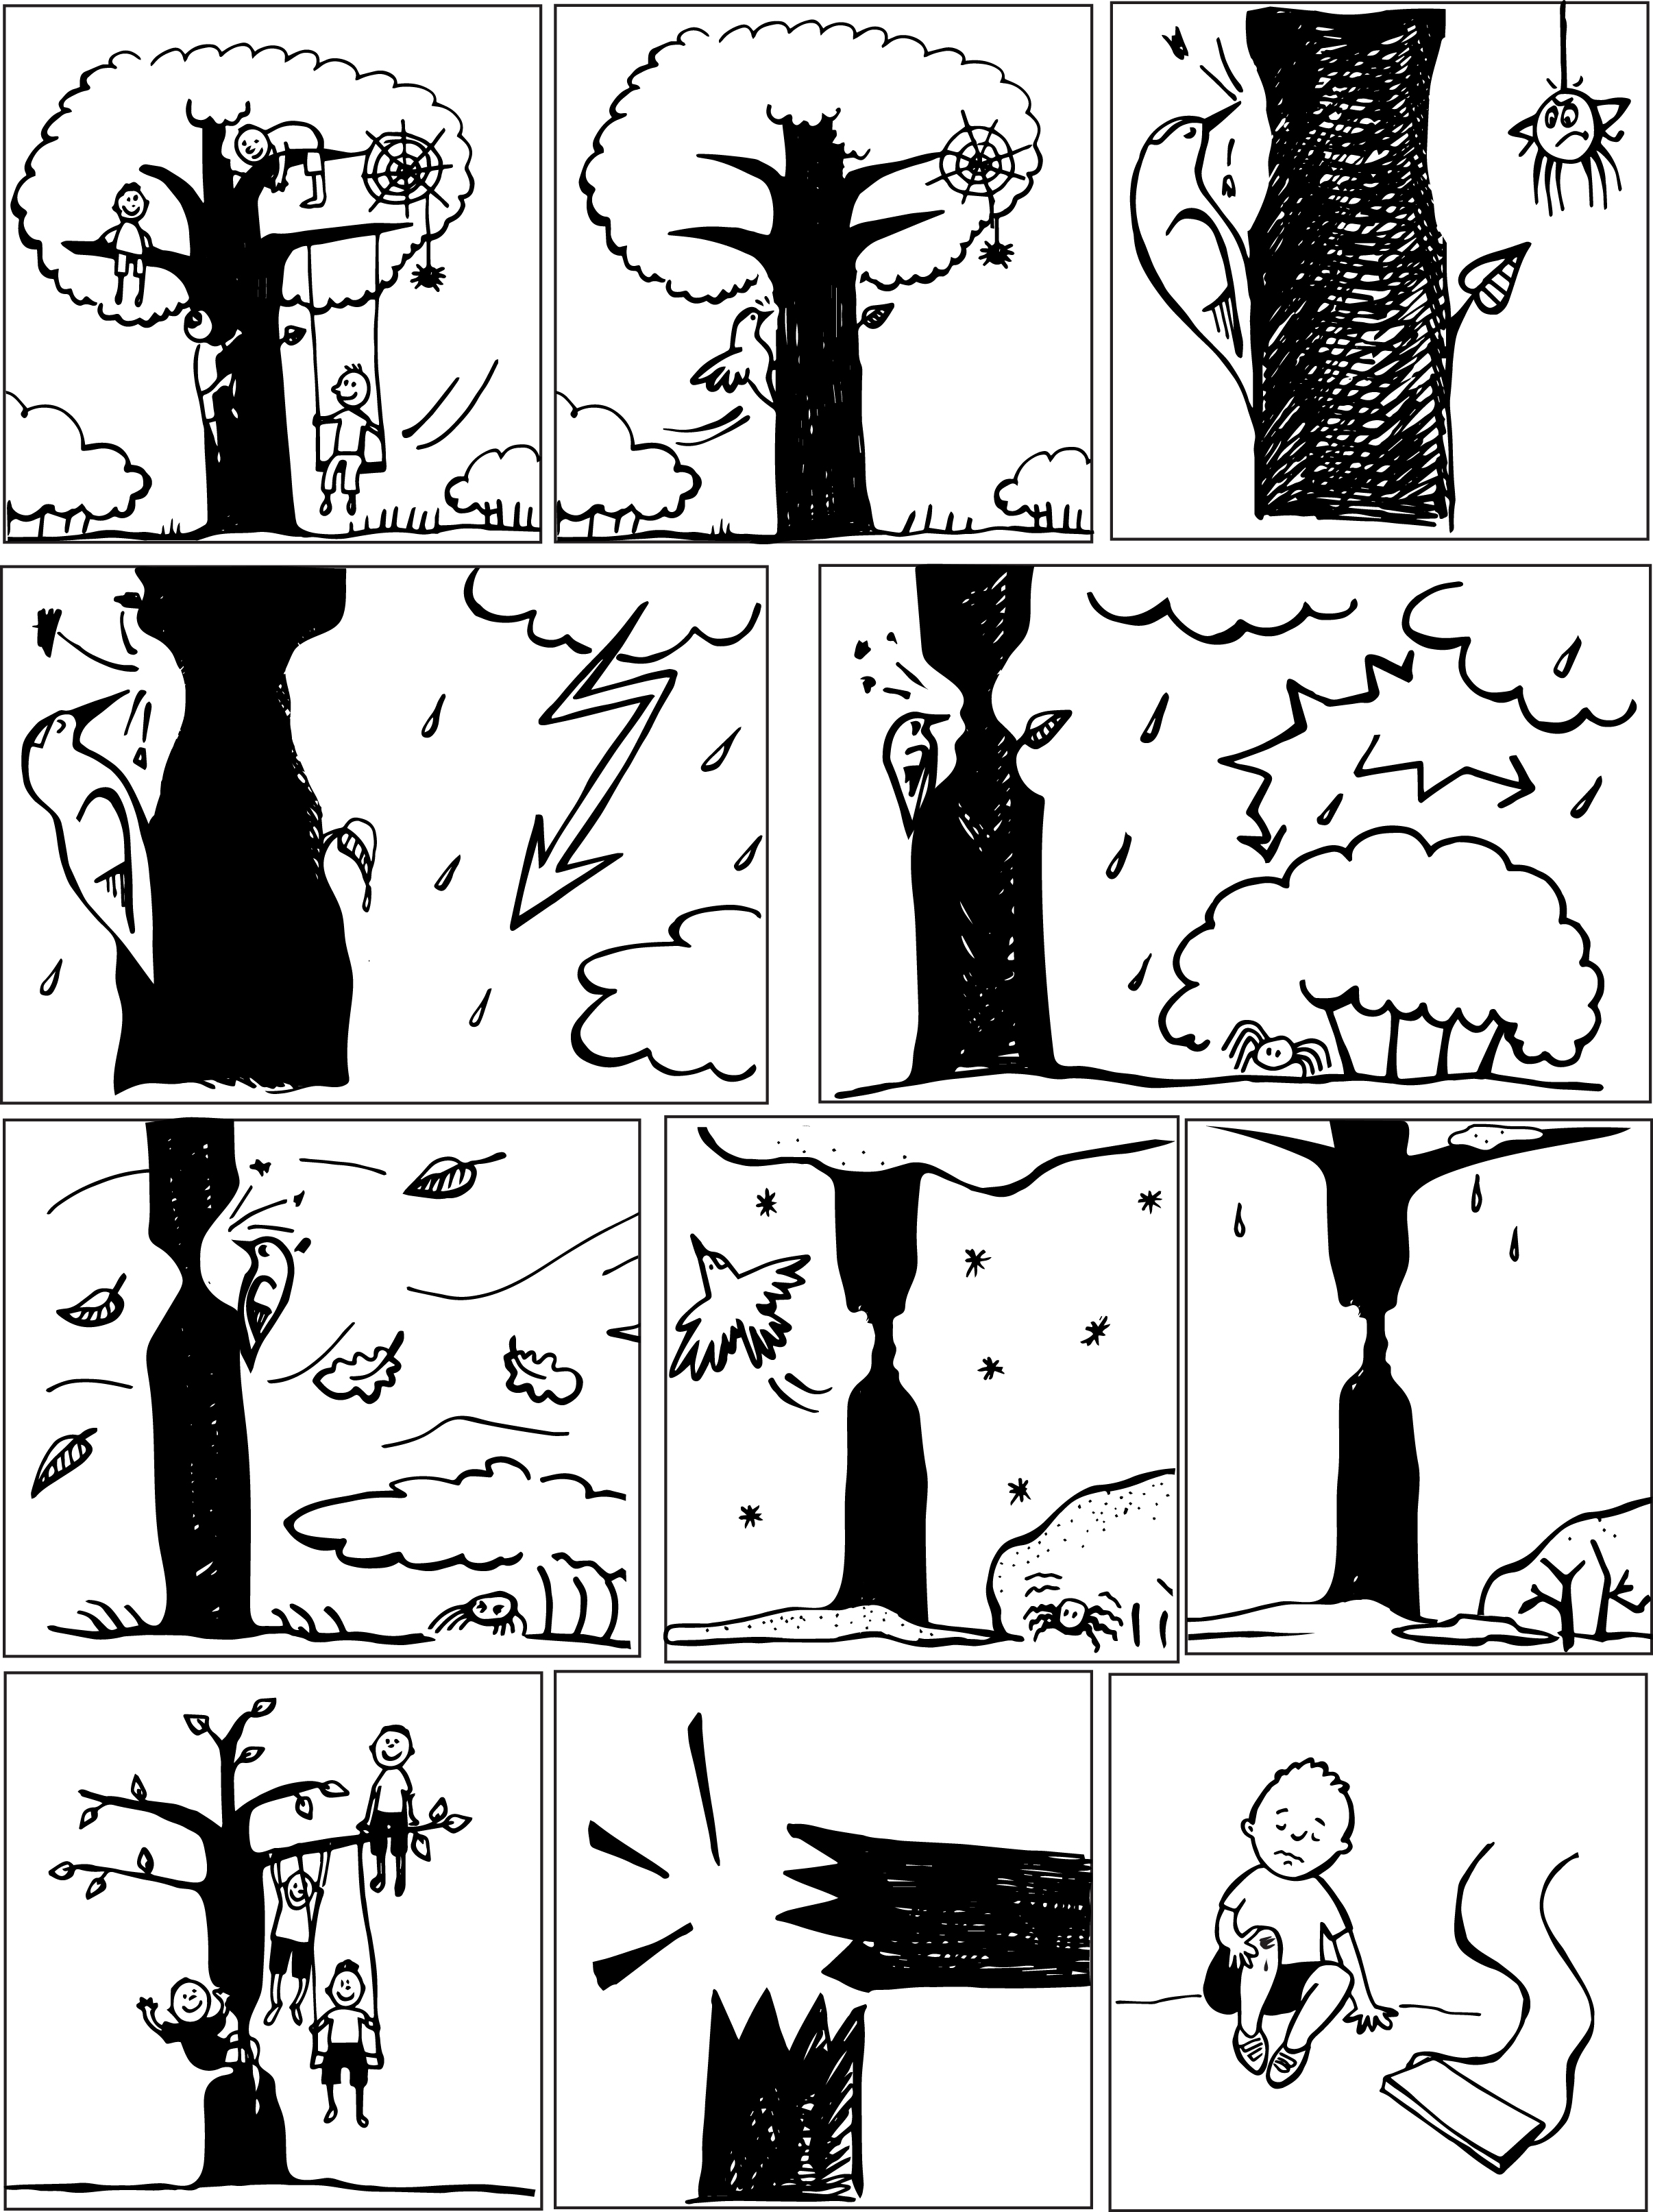
\includegraphics[width=\linewidth]{pauk.jpg}\\
\pagebreak\\
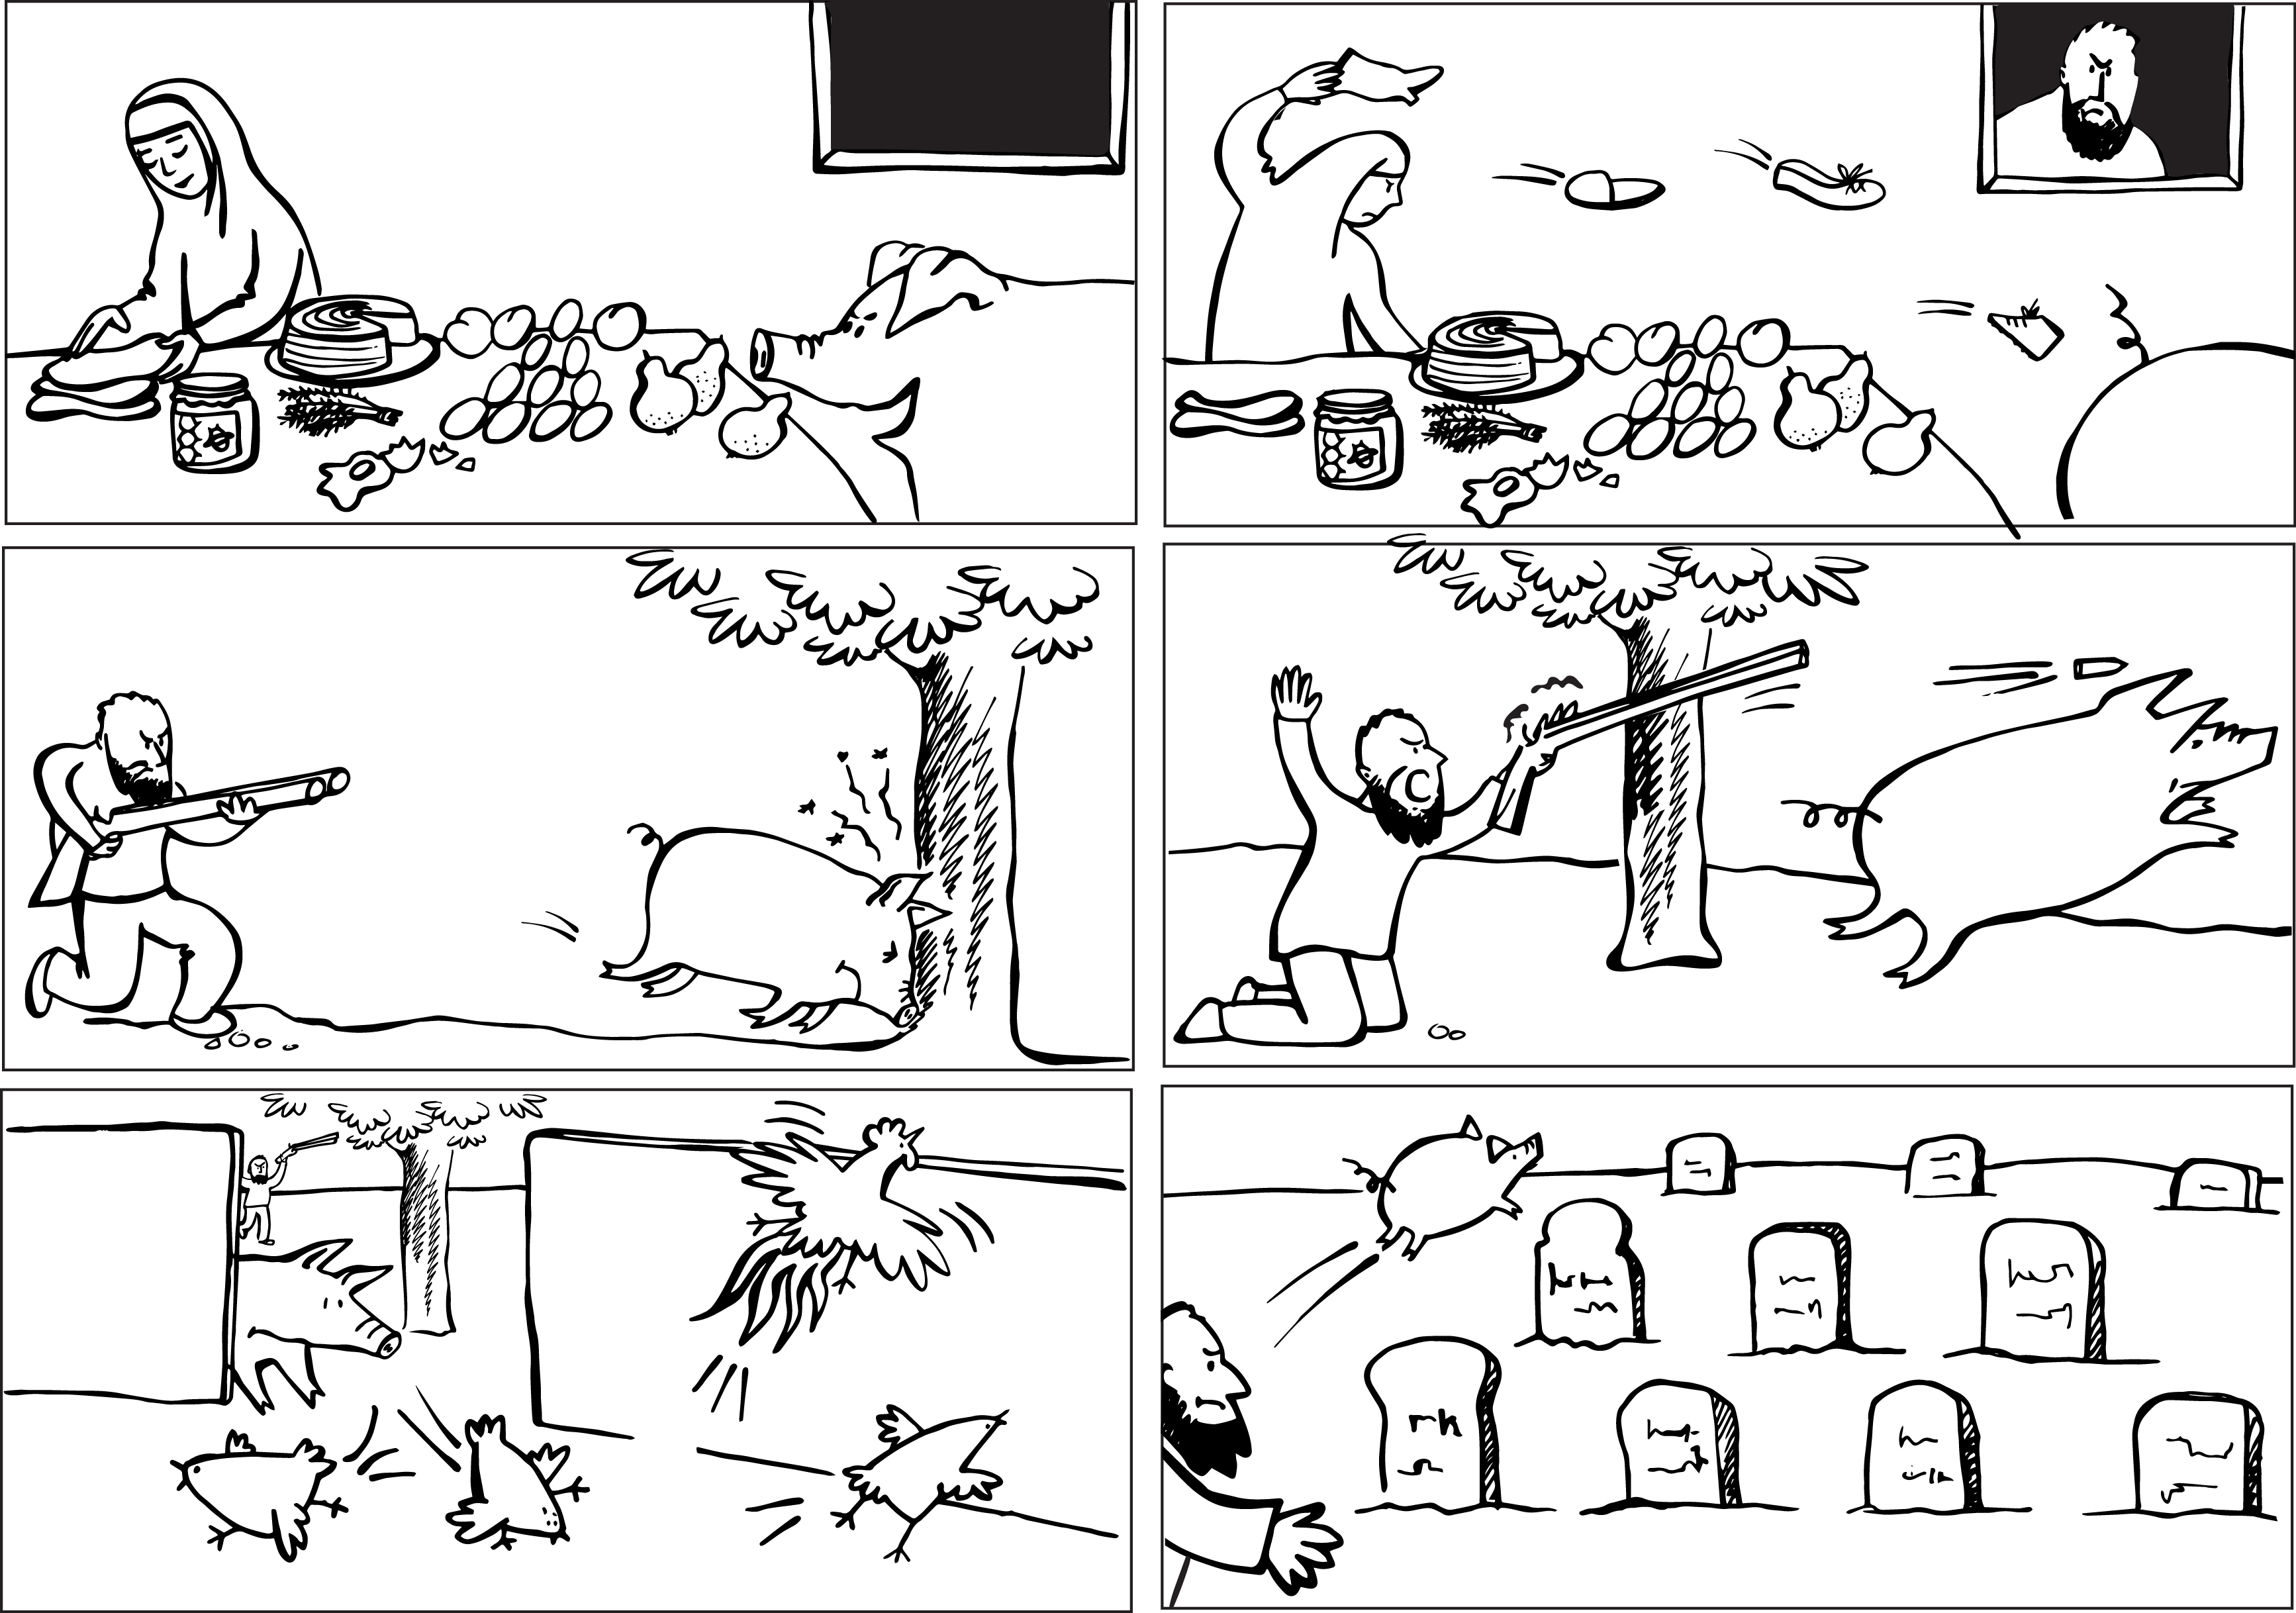
\includegraphics[width=\linewidth]{svinja.jpg}\\
\pagebreak
\subsection{Приложение 2: стихотворение Алима Кешокова} \label{verse}
\noindent Текст оригинального стихотворения Алима Кешокова пришлось значительно переделать, чтобы оно соответствовало лексике и грамматике кубанского говора, а также приблизить его к орфографии адыгейского языка, к которой привыкли носители. Ниже приводятся оригинал и получившийся в результате текст, который давался информантам:
\begin{multicols}{2}
\noindent оригинал \medskip\\
Зыхэс удз Iувыр ирецIынэ,\\
И Iэщхьэр лъагэу дэхьеяуэ\\
Хъыджэбз нэкIуплъым епщ хупцIынэ,\\
Щхьэщысщ ар Iэнлъэм зигъэщхъауэ.\medskip\\
ЕIуящIэ защIэу щIалэ куэди\\
КъетIысэкIауэ мэгушыIэ.\\
И уз а пщафIэми укIуэди,\\
Сыт къыхуапсэлъми зешыIэ.\medskip\\
ТIэкIу зигъэщхъакъэ --- псори маплъэ,\\
А щIалэр зэплъыр къыпхуэмыщIэ,\\
Хъыджэбзырз зыщIэр псом я пIалъэ\\
Зигу къэплъым и Iур ирегъущIэ. \medskip\\
И щхьэцыр пщащэм ирекъуэкIыр,\\
Хьэжыгъэр нэIум къытощащэ.\\
Гу лъумытэну я гум къэкIым,\\
ЩIалэжьхэр къеплъмэ, мэIущащэ.\medskip\\ 
Я мэлхэр шытхым щхьэдэхами,\\
Мэлыхъуэр зыкIи мыгузавэ.\\
Дэтхэнэм жьэкIэ сыт жиIами,\\
Я плъырыр псалъэм щIрагъавэ.\medskip\\
Зырыз мэл хъушэу къыдахуащ,\\
АрщхьэкIэ псоми зыщ ягъэхъур.\\
А хъыджэбз пщафIэм дихьэхащ --- \\
Апхуэдэу махуэр жэщ ягъэхъур. \medskip\\
Сыт щIалэ жанхэри зезыхьэр?\\
Мэлыхъуэм я гур хьэхугъуафIэщ,\\
Хъыджэбзым ищIрэ щIакхъуэ Iыхьэ,\\
Iухуакъэ, ишхыр хъунущ мафIэ.\\
\columnbreak\\
\noindent результат обработки \medskip\\
Зыхэс удз Iувыр ирецIынэ,\\
И Iэшъхьэр лъагу дэхьэяуэ \\
Хъыджэбз нэкIуплъым епшъ тхьавыщхуэ,\\
Шъхьэшъыс ар табэм итхьэшIауэ. \medskip\\
Iэнэщхуэ шIами шIэлэ коди\\
КъетIысэкIао уэрэд жьаIэ\\
Иуз а пшъафIэм ирекIоди,\\
Сыт хужьаIами зещыIэ.\medskip\\
ТIэкIу зауыхуакъэ  --- пстори маплъэ, \\
А шIалэр здэплъэр къомыцIыху, \\
Хъыджэбзым декIэ пстори маплъэ --- \\
Зигу къэплъым иIур ёгъушъыкI. \medskip\\
Ишъхьэцыр пшъашъэм иредзэкI,\\
Хьэжьыгъэр нэкIум къытошъашъэ.\\
Гу лъомытэну ягум къэкIым,\\
ШIалэжъхэр къеплъмэ мэIушъашъэ.\medskip\\
Ямэлхэр джабэм дагъэкIами,\\
Мэлахъуэр зыкIи мыгузавэ.\\
Зыгуэрэ жъэкIэ сыт жьиIами,\\
Мэлахъуэр псалъэм шIырагъавэ.\medskip\\
Мин дапшъэ мэлу къыдахуа,\\
А шъхьэкIэ пстоми зы ягъэхъу.\\
А хъыджэбз пшъафIэм дихьэха --- \\
Апхуэду махуэр жьэщ ягъэхъу. \medskip\\
Сыт шIалэ жьанхэри зезыхьэр?\\
Мэлыхъуэм игур кIуэдыгъуафIэ,\\
Хъыджэбзым ишIрэ шIакъуэ Iыхьэ,\\
Iухуакъэ, ищхыр хъунэ мафIэ.\\
\end{multicols}
\textit{Алим КIышъокъо, Тхыгъэхэр, томихым шъызэхохьэсао ---  Налшъык: <<Эльбрус>>, 2004. --- н. 147}
\pagebreak	
\subsection{Приложение 3: прозаический текст} \label{text}
\noindent При чтении прозаического фрагмента использовалась история составленная с информантами: \medskip\\
\noindent Зы махуэ гуэрэм сэ Лабинск сыкIуэт. Хуэбэ Iет. Маршруткэм сису, жъышIэхуыр сIыгъу жъы сеуэт. Телефоныр къытеуа. Телефоныр къытесха ар Аслъэн къэзышIыр.\\
– Дыгъуасэ, уэ си машинэ IункIыбзэр Аминэрэ Бислъанрэ ириджэгуну яптатэкъэ? – жьери къызэуыпшIа.\\
– Ае, – жьесIэжьа.\\
– Тэнэ ар здахьар?\\
– Уэуи, сабихэр пщахъуэм шъыджэгуахэт, абым къыханауэ шътын. Уынэм къышъышIэхьэжьхэм уиIункIыбзэр яIыгъу слъэгъуакъым.\\
– Тэнэ джы здэкIуар тIэ сиIункIыбзэр? – Аслъан  къышIэуыпшIа.\\
– Тэнэ сэ шъысцIыхуыр? Нэнаухэм пщахъуэм Аслъан иIункIыбзэр шIэтIтIат жьаIу къызжьаIа пфIэшIрэ?\\
– ПсынчIу, псынчIу къэгъуэтыжь, сэ Майкоп сыкIуэн хует нэIэ джыпсту, шъхьакIэ сиIункIыбзэр вгъэкIуэда.\\
– Ой сэ Лабинск сокIуэ джыпсту, къысхуэгъэгъу. Сиде Iуыхьи, уынэм шIыхьи сабихэм яупшI. КъагъуэтыжьынкIи мэхъу.\bigskip\\

\textbf{Перевод:}\\
Однажды я ехала в Лабинск. Жара стращная. Я сижу в маршрутке, в руках веер, обмахиваюсь. Тут телефон звонит. Оказалось это Аслан.\\
--- Ты давала вчера мои ключи от машины Амине и Бислану поиграть? --- спросил он.\\
--- Да, --- отвечаю.\\
--- Ну и куда они их дели?\\
--- Ой, дети играли в песочнице, там, наверное, и оставили. Я не видела ключей, когда они в дом зашли.\\
--- Ну и где тогда теперь мои ключи?\\
--- Откуда я знаю? Думаешь, они пришли и сказали "мы закопали ключи Аслана".
--- Быстрее, быстрее, найди их, я же в Майкоп поехать не могу, из-за того, что вы ключи потеряли.\\
--- Ой, я в Лабинск сейчас еду, прости. Ко мне домой зайди, детей спроси. Может найдутся.
\pagebreak
\subsection{Приложение 4: скрипт в Praat (v. 5.3.16)} \label{praatscript}
\noindent Данный скрипт был написан Mietta Lennes, однако я несколько изменил его для своего удобства. Теперь он вытаскивает название всех фрагментов (в случае паузы название отсутствует), длительность, время начала фрагмента и время конца фрагмента.
\scriptsize
\begin{alltt}
# This script is distributed under the GNU General Public License.
# Copyright 12.3.2002 Mietta Lennes

# ask the user for the tier number
form Calculate durations of labeled segments
	comment Which tier of the TextGrid object would you like to analyse?
	integer Tier 1
	comment Where do you want to save the results?
	text informant D3
	text textfile /home/.../durations_of_D3.txt
endform

# check how many intervals there are in the selected tier:
numberOfIntervals = Get number of intervals... tier

# loop through all the intervals
for interval from 1 to numberOfIntervals
	label$ = Get label of interval... tier interval
	# if the interval has some text as a label, then calculate the duration.
	if label$ <> ""
		start = Get starting point... tier interval
		end = Get end point... tier interval
		duration = (end - start)*1000
		# append the label and the duration to the end of the text file, separated with a tab:		
		resultline$ = "'informant$''tab$''label$''tab$''duration''tab$''start''tab$''end''newline$'"
		fileappend "'textfile$'" 'resultline$'
	endif
endfor

# the end of the script
\end{alltt}
\normalsize
\pagebreak
\subsection{Приложение 5: код в R (v. 3.3.1)} \label{Rscript}
\noindent Данный скрипт принимает на вход данные полученные скриптом Praat и считает результаты для рисунка \ref{verseboxplot}.
\scriptsize
\begin{alltt}
df <- read.csv("https://goo.gl/tz50SW", sep = "\t", header = F)
names(df) <- c("dictor",
               "number.of.syllables",
               "duration",
               "start",
               "end")

dfall <- df
dfall$dictor <- "all"
dfall <- rbind.data.frame(df, dfall)

articulation.rate <- cbind.data.frame(dfall$dictor, dfall$number.of.syllables/dfall$duration*1000)
names(articulation.rate) <- c("dictor", "art.rate")
rate.speaker <- c(by(articulation.rate$art.rate, articulation.rate$dictor, mean))
rate.speaker <- as.data.frame(rate.speaker)
rate.speaker$ci <- c(by(articulation.rate$art.rate, articulation.rate$dictor, 
                        function(x){1.96*sd(x)/sqrt(length(x))}))
rate.speaker$sd <- c(by(articulation.rate$art.rate, articulation.rate$dictor, 
                        sd))

library(ggplot2)
ggplot(dfall, aes(dictor, number.of.syllables/duration*1000))+
  geom_boxplot()+
  ylab("количество слогов в секунду")+
  xlab("диктор")+
  ggtitle("Скорость чтения стихотворения")+
  theme_bw()
\end{alltt}
\normalsize
\noindent Данный скрипт принимает на вход данные полученные скриптом Praat и считает результаты для рисунка \ref{proseboxplot}.
\scriptsize
\begin{alltt}
setwd("/home/agricolamz/_DATA/OneDrive1/_Work/_Handouts/2016 II Adyghe expedition/audio")
df <- read.csv("durations_of_prose.txt", sep = "\t", header = F)
names(df) <- c("dictor",
               "number.of.syllables",
               "duration",
               "start",
               "end")

dfall <- df
dfall$dictor <- "all"
dfall <- rbind.data.frame(df, dfall)

articulation.rate <- cbind.data.frame(dfall$dictor, dfall$number.of.syllables/dfall$duration*1000)
names(articulation.rate) <- c("dictor", "art.rate")
rate.speaker <- c(by(articulation.rate$art.rate, articulation.rate$dictor, mean))
rate.speaker <- as.data.frame(rate.speaker)
rate.speaker$ci <- c(by(articulation.rate$art.rate, articulation.rate$dictor, 
                        function(x){1.96*sd(x)/sqrt(length(x))}))
rate.speaker$sd <- c(by(articulation.rate$art.rate, articulation.rate$dictor, 
                        sd))


library(ggplot2)
ggplot(dfall, aes(dictor, number.of.syllables/duration*1000))+
  geom_boxplot()+
  ylab("количество слогов в секунду")+
  xlab("диктор")+
  ggtitle("Скорость чтения прозаического текста")+
  theme_bw()
# the end of the script
\end{alltt}
\normalsize
\pagebreak
\subsection{Приложение 6: разбор записанных нарративов} \label{corpus}
\bpaformat{1}{(}{\_D1)}
\lbpa{}{\gll zə maxʷe gʷere-m ...(0.3) fəzə-m ...(1.2) pješ'ḳe  jə-ʁe-ẑe-n-u ...(0.4) r-jə-qʷəh-a\\
один день \textsc{indef-obl} \textsc{hes} женшина-\textsc{obl} \textsc{hes} пышка \textsc{3sg.erg-caus}-жариться-\textsc{mod-adv} \textsc{hes} \textsc{dat-3sg.erg}-собираться-\textsc{pst}\\
\trans `Однажды женщина собралась пожарить пышки' \hfill (00:01.726--00:08.047)}

\lbpa{}{\gll pjəš'ḳe jə-ʁe-ẑe-nə-m= ee(0.8) jə-ʁa-ẑe ...(0.1) petre ...(0.9) qχʷje= məst qχʷe qə-ʔʷə-h-a\\
пышка 3sg.\textsc{erg-caus}-жариться-\textsc{mod-obl} \textsc{hes} \textsc{3sg.erg-caus}-жариться \textsc{hes} когда \textsc{hes} сыр= \textsc{filler} свинья \textsc{dir-loc}-входить-\textsc{pst}\\
\trans `Только-только собралась пожарить пышки' \hfill (00:09.535--00:15.976)}

\lbpa{}{\gll qχʷe\\
свинья\\
\trans `Свинья' \hfill (00:16.333--00:16.714)}

\lbpa{}{\gll qχʷe-r= fəzə-m qχʷe-r ...(0.1) jə-r-jə-xʷəẑ-a \\
свинья-\textsc{abs} женщина-\textsc{obl} свинья-\textsc{abs} \textsc{hes} \textsc{loc-dat-3sg.erg}-прогнать-\textsc{pst}\\
\trans `Свинья... Женщина прогнала свинью' \hfill (00:20.964--00:26.166)}

\lbpa{}{\gll vaqe-r q-jə-ŝte-rjə vaqe-m-č̣'e č̣'e.ɬə-w-re ...(0.1) qχʷe-r jə-r-jə-xʷəẑ-a \\
обувь-\textsc{abs} \textsc{dir-3sg.erg}-взять-\textsc{cvb} обувь-\textsc{obl-ins} \textsc{loc}-бить-\textsc{cvb} \textsc{hes} свинья-\textsc{abs} \textsc{loc-dat-3sg.erg}-прогнать-\textsc{pst} \\
\trans `Взяла обувь и обувью прогнала' \hfill (00:26.714--00:30.702)}

\lbpa{}{\gll jəṭane qə= ...(0.1) qə-z-d-jə-č̣'-a-r-jə sə-mə-cəxʷ-u ɬ̣ə gʷəre qə-ʔʷə-h-a \\
потом \textsc{dir}= \textsc{hes} \textsc{dir-rel.io-loc-3sg.erg}-прийти-\textsc{pst-abs-add} \textsc{1sg.abs-neg}-знать-\textsc{adv} мужчина \textsc{indef} \textsc{dir-loc}-входить-\textsc{pst}\\
\trans `Потом откуда ни возьмись какой-то мужчина подошел' \hfill (00:31.44--00:34.42)}

\lbpa{}{\gll məst ɬ̣ə-m fonč'ə-r ...(0.1) jə-ŝte-rjə ...(0.8) a qχʷe-m  č̣'e.ɬə-w-a\\
\textsc{filler} мужчина-\textsc{obl} ружье-\textsc{abs} \textsc{hes} \textsc{3sg.abs}-взять-\textsc{cvb} \textsc{hes} тот свинья-\textsc{obl} \textsc{loc}-бить-\textsc{pst}\\
\trans `Взял ружье и выстрелил в свинью' \hfill (00:34.433--00:39.333)}

\lbpa{}{\gll č̣'e.ɬə-w-a ŝhač̣'e tər-jə-ʁe-xʷe-f-a-qəm, ...(0.6) jəṭane-č̣'e ee(0.9) ǯ'ed-xe-[rə]-m-re ...(0.6) adaqe gʷere-re qə-qʷe-č̣'-a-xe \\
\textsc{loc}-бить-\textsc{pst} но \textsc{loc-3sg.erg-caus}-упасть-\textsc{pot-pst-neg} \textsc{hes} потом-\textsc{ins} \textsc{hes} курица-\textsc{pl-[???]-obl-coord} \textsc{hes} петух \textsc{indef-coord} \textsc{dir-loc}-выходить-\textsc{pst-pl} \\
\trans `Выстрелил, но не мог попасть, потом курицы и какой-то петух вышли' \hfill (00:40.458--00:48.082)}

\lbpa{}{\gll ɬ̣ə-m ač̣'= ee(0.5) qχʷe-r jə-ra-xʷəẑe ŝebjə-m-č̣'-jə ee(1.7) qχe-m nes-č̣e ja-xʷ-a \textbf{\textit{i}} ...(0.9) qχʷe-r ...(1.0) qχe-m-č̣'e ...(0.4) ble-č̣'-a z-de-ḳʷ-a-r-jə s-c̣əxʷ-qəm   \\     
мужчина-\textsc{obl} = \textsc{hes} свинья-\textsc{abs} \textsc{dat-3pl.erg}-гнать потом-\textsc{obl-ins-add} \textsc{hes} кладбище-\textsc{obl} до-\textsc{ins 3pl.erg}-гнать-\textsc{pst} и \textsc{hes} свинья-\textsc{abs}  \textsc{hes} кладбище-\textsc{obl-ins hes loc}-выходить-\textsc{pst} \textsc{rel.io-loc}-идти-\textsc{pst-abs-add} \textsc{1sg.erg}-знать-\textsc{neg}\\
\trans `За свиньей погнались, гнали до кладбища,  свинья прошла кладбище, куда пошла не знаю' \\ \hfill(00:51.706--01:02.844)}

\bpaformat{1}{(}{\_D2)}

\pagebreak
\subsection{Приложение 7: raw data для исследования длительности нарративов} \label{corpus.raw}
\pagebreak
\subsection{Приложение 8: raw data для исследования длительности в стихах} \label{verse.raw}
\begin{longtable}{|l|l|l|l|l|}
\hline
диктор & количество слогов & длительность (мс) & время начала (с) & время конца (с)\\
\hline \endhead
D1 & 9 & 2480 & 1.46 & 3.94 \\ \hline
D1 & 9 & 2330 & 4.06 & 6.39 \\ \hline
D1 & 9 & 2550 & 6.71 & 9.26 \\ \hline
D1 & 9 & 2330 & 9.6 & 11.93 \\ \hline
D1 & 9 & 2320.0000000000005 & 12.42 & 14.74 \\ \hline
D1 & 9 & 2069.9999999999986 & 15.06 & 17.13 \\ \hline
D1 & 9 & 2320.0000000000005 & 17.68 & 20 \\ \hline
D1 & 8 & 1849.999999999998 & 20.26 & 22.11 \\ \hline
D1 & 9 & 2660 & 22.8 & 25.46 \\ \hline
D1 & 9 & 2320.0000000000005 & 25.72 & 28.04 \\ \hline
D1 & 9 & 2350.0000000000014 & 28.38 & 30.73 \\ \hline
D1 & 8 & 2230.0000000000005 & 30.95 & 33.18 \\ \hline
D1 & 8 & 2049.9999999999973 & 33.74 & 35.79 \\ \hline
D1 & 9 & 2280.000000000001 & 36.22 & 38.5 \\ \hline
D1 & 9 & 2090.0000000000036 & 38.69 & 40.78 \\ \hline
D1 & 9 & 2399.9999999999986 & 41.02 & 43.42 \\ \hline
D1 & 9 & 2260.000000000005 & 43.76 & 46.02 \\ \hline
D1 & 9 & 2200.0000000000027 & 46.3 & 48.5 \\ \hline
D1 & 9 & 2109.9999999999995 & 48.82 & 50.93 \\ \hline
D1 & 9 & 2219.999999999999 & 51.18 & 53.4 \\ \hline
D1 & 8 & 2169.9999999999945 & 53.81 & 55.98 \\ \hline
D1 & 8 & 2309.999999999995 & 56.34 & 58.65 \\ \hline
D1 & 8 & 2090.0000000000036 & 59.22 & 61.31 \\ \hline
D1 & 8 & 2109.9999999999995 & 61.58 & 63.69 \\ \hline
D1 & 9 & 2349.9999999999945 & 64.17 & 66.52 \\ \hline
D1 & 9 & 2099.9999999999945 & 66.81 & 68.91 \\ \hline
D1 & 11 & 3569.999999999993 & 69.12 & 72.69 \\ \hline
D1 & 9 & 2500 & 73.16 & 75.66 \\ \hline
D1 & 9 & 2480 & 1.46 & 3.94 \\ \hline
D1 & 9 & 2330 & 4.06 & 6.39 \\ \hline
D1 & 9 & 2550 & 6.71 & 9.26 \\ \hline
D1 & 9 & 2330 & 9.6 & 11.93 \\ \hline
D1 & 9 & 2320.0000000000005 & 12.42 & 14.74 \\ \hline
D1 & 9 & 2069.9999999999986 & 15.06 & 17.13 \\ \hline
D1 & 9 & 2320.0000000000005 & 17.68 & 20 \\ \hline
D1 & 8 & 1849.999999999998 & 20.26 & 22.11 \\ \hline
D1 & 9 & 2660 & 22.8 & 25.46 \\ \hline
D1 & 9 & 2320.0000000000005 & 25.72 & 28.04 \\ \hline
D1 & 9 & 2350.0000000000014 & 28.38 & 30.73 \\ \hline
D1 & 8 & 2230.0000000000005 & 30.95 & 33.18 \\ \hline
D1 & 8 & 2049.9999999999973 & 33.74 & 35.79 \\ \hline
D1 & 9 & 2280.000000000001 & 36.22 & 38.5 \\ \hline
D1 & 9 & 2090.0000000000036 & 38.69 & 40.78 \\ \hline
D1 & 9 & 2399.9999999999986 & 41.02 & 43.42 \\ \hline
D1 & 9 & 2260.000000000005 & 43.76 & 46.02 \\ \hline
D1 & 9 & 2200.0000000000027 & 46.3 & 48.5 \\ \hline
D1 & 9 & 2109.9999999999995 & 48.82 & 50.93 \\ \hline
D1 & 9 & 2219.999999999999 & 51.18 & 53.4 \\ \hline
D1 & 8 & 2169.9999999999945 & 53.81 & 55.98 \\ \hline
D1 & 8 & 2309.999999999995 & 56.34 & 58.65 \\ \hline
D1 & 8 & 2090.0000000000036 & 59.22 & 61.31 \\ \hline
D1 & 8 & 2109.9999999999995 & 61.58 & 63.69 \\ \hline
D1 & 9 & 2349.9999999999945 & 64.17 & 66.52 \\ \hline
D1 & 9 & 2099.9999999999945 & 66.81 & 68.91 \\ \hline
D1 & 11 & 3569.999999999993 & 69.12 & 72.69 \\ \hline
D1 & 9 & 2500 & 73.16 & 75.66 \\ \hline
D2 & 9 & 2400 & 2.89 & 5.29 \\ \hline
D2 & 9 & 2419.999999999999 & 5.7 & 8.12 \\ \hline
D2 & 9 & 2929.9999999999995 & 8.435 & 11.365 \\ \hline
D2 & 9 & 2429.9999999999995 & 11.815 & 14.245 \\ \hline
D2 & 9 & 2910 & 15.335 & 18.245 \\ \hline
D2 & 9 & 2330.000000000002 & 18.985 & 21.315 \\ \hline
D2 & 9 & 2539.999999999999 & 21.555 & 24.095 \\ \hline
D2 & 8 & 2619.9999999999973 & 24.53 & 27.15 \\ \hline
D2 & 9 & 3209.9999999999973 & 27.6 & 30.81 \\ \hline
D2 & 8 & 3010.0000000000014 & 31.16 & 34.17 \\ \hline
D2 & 9 & 2564 & 34.467 & 37.031 \\ \hline
D2 & 8 & 2903.9999999999964 & 37.392 & 40.296 \\ \hline
D2 & 8 & 2403.9999999999964 & 41.094 & 43.498 \\ \hline
D2 & 9 & 2063.0000000000023 & 44.28 & 46.343 \\ \hline
D2 & 9 & 2447.0000000000027 & 46.775 & 49.222 \\ \hline
D2 & 9 & 3213.000000000001 & 49.641 & 52.854 \\ \hline
D2 & 9 & 2777.000000000001 & 53.669 & 56.446 \\ \hline
D2 & 9 & 2893.999999999998 & 56.902 & 59.796 \\ \hline
D2 & 9 & 3809.0000000000045 & 60.29 & 64.099 \\ \hline
D2 & 9 & 2521.000000000001 & 64.401 & 66.922 \\ \hline
D2 & 8 & 2605.9999999999945 & 67.73 & 70.336 \\ \hline
D2 & 8 & 2435.9999999999927 & 71.102 & 73.538 \\ \hline
D2 & 8 & 2680.9999999999973 & 74.006 & 76.687 \\ \hline
D2 & 9 & 2521.000000000001 & 77.181 & 79.702 \\ \hline
D2 & 9 & 4606.999999999999 & 80.988 & 85.595 \\ \hline
D2 & 9 & 3277.000000000001 & 85.978 & 89.255 \\ \hline
D2 & 9 & 3713.000000000008 & 89.743 & 93.456 \\ \hline
D2 & 8 & 3807.9999999999927 & 95.265 & 99.073 \\ \hline
D3 & 9 & 2720.0000000000005 & 3.26 & 5.98 \\ \hline
D3 & 11 & 3290.000000000001 & 7.1 & 10.39 \\ \hline
D3 & 9 & 3130.000000000001 & 10.67 & 13.8 \\ \hline
D3 & 9 & 2409.999999999998 & 14.74 & 17.15 \\ \hline
D3 & 9 & 2840 & 18.3 & 21.14 \\ \hline
D3 & 9 & 2660 & 22 & 24.66 \\ \hline
D3 & 9 & 2590 & 25.53 & 28.12 \\ \hline
D3 & 8 & 2570.0000000000005 & 28.94 & 31.51 \\ \hline
D3 & 11 & 4250 & 33.05 & 37.3 \\ \hline
D3 & 9 & 3020.000000000003 & 37.87 & 40.89 \\ \hline
D3 & 9 & 2795.000000000002 & 41.375 & 44.17 \\ \hline
D3 & 8 & 3020.000000000003 & 44.76 & 47.78 \\ \hline
D3 & 8 & 2369.9999999999973 & 48.59 & 50.96 \\ \hline
D3 & 9 & 2659.9999999999964 & 51.59 & 54.25 \\ \hline
D3 & 8 & 2549.9999999999973 & 54.84 & 57.39 \\ \hline
D3 & 9 & 2630.0000000000027 & 58 & 60.63 \\ \hline
D3 & 9 & 2469.999999999999 & 61.58 & 64.05 \\ \hline
D3 & 9 & 2830.0000000000127 & 64.6 & 67.43 \\ \hline
D3 & 9 & 3079.999999999998 & 68.04 & 71.12 \\ \hline
D3 & 9 & 2689.9999999999977 & 71.4 & 74.09 \\ \hline
D3 & 11 & 3060.0000000000023 & 74.8 & 77.86 \\ \hline
D3 & 9 & 3150.0000000000055 & 79.03 & 82.18 \\ \hline
D3 & 8 & 2430.000000000007 & 82.77 & 85.2 \\ \hline
D3 & 9 & 2820.0000000000073 & 85.88 & 88.7 \\ \hline
D3 & 9 & 2689.9999999999977 & 89.78 & 92.47 \\ \hline
D3 & 9 & 3010.000000000005 & 93.1 & 96.11 \\ \hline
D3 & 9 & 3370.0000000000045 & 96.6 & 99.97 \\ \hline
D3 & 9 & 3689.9999999999977 & 101.11 & 104.8 \\ \hline
D4 & 9 & 2430 & 3.82 & 6.25 \\ \hline
D4 & 9 & 2210 & 6.54 & 8.75 \\ \hline
D4 & 9 & 2629.999999999999 & 9.05 & 11.68 \\ \hline
D4 & 9 & 2639.9999999999986 & 11.98 & 14.62 \\ \hline
D4 & 9 & 2299.999999999999 & 15.135 & 17.435 \\ \hline
D4 & 9 & 2230.0000000000005 & 17.84 & 20.07 \\ \hline
D4 & 9 & 2160 & 20.44 & 22.6 \\ \hline
D4 & 8 & 2210.000000000001 & 22.915 & 25.125 \\ \hline
D4 & 9 & 2530.000000000001 & 25.625 & 28.155 \\ \hline
D4 & 8 & 2050.000000000001 & 28.48 & 30.53 \\ \hline
D4 & 9 & 2499.9999999999964 & 31.01 & 33.51 \\ \hline
D4 & 8 & 2450.0000000000027 & 33.885 & 36.335 \\ \hline
D4 & 9 & 2480.000000000004 & 36.86 & 39.34 \\ \hline
D4 & 9 & 2399.9999999999986 & 39.585 & 41.985 \\ \hline
D4 & 9 & 2399.9999999999986 & 42.33 & 44.73 \\ \hline
D4 & 9 & 2579.999999999998 & 44.975 & 47.555 \\ \hline
D4 & 9 & 2400.0000000000055 & 48.16 & 50.56 \\ \hline
D4 & 9 & 2179.9999999999995 & 51.005 & 53.185 \\ \hline
D4 & 9 & 2189.9999999999977 & 53.56 & 55.75 \\ \hline
D4 & 9 & 2500 & 56.05 & 58.55 \\ \hline
D4 & 8 & 2049.9999999999973 & 59.13 & 61.18 \\ \hline
D4 & 8 & 2239.999999999995 & 61.67 & 63.91 \\ \hline
D4 & 8 & 2150.0000000000055 & 64.27 & 66.42 \\ \hline
D4 & 8 & 2319.999999999993 & 66.81 & 69.13 \\ \hline
D4 & 8 & 2250 & 69.6 & 71.85 \\ \hline
D4 & 9 & 2159.9999999999964 & 72.41 & 74.57 \\ \hline
D4 & 9 & 2280.000000000001 & 74.965 & 77.245 \\ \hline
D4 & 9 & 2460.000000000008 & 77.63 & 80.09 \\ \hline
D5 & 9 & 2199.9999999999995 & 2.02 & 4.22 \\ \hline
D5 & 9 & 2140.0000000000005 & 4.56 & 6.7 \\ \hline
D5 & 9 & 2460.000000000001 & 7 & 9.46 \\ \hline
D5 & 9 & 2250 & 9.72 & 11.97 \\ \hline
D5 & 9 & 2060.0000000000005 & 12.49 & 14.55 \\ \hline
D5 & 9 & 1970.0000000000007 & 14.755 & 16.725 \\ \hline
D5 & 9 & 2359.9999999999995 & 17.045 & 19.405 \\ \hline
D5 & 9 & 2039.999999999999 & 19.57 & 21.61 \\ \hline
D5 & 9 & 4230 & 22.34 & 26.57 \\ \hline
D5 & 9 & 2420.000000000002 & 26.83 & 29.25 \\ \hline
D5 & 9 & 2229.999999999997 & 29.6 & 31.83 \\ \hline
D5 & 8 & 2399.9999999999986 & 32.1 & 34.5 \\ \hline
D5 & 8 & 2009.999999999998 & 35.32 & 37.33 \\ \hline
D5 & 9 & 1969.9999999999989 & 37.68 & 39.65 \\ \hline
D5 & 9 & 2250 & 40.02 & 42.27 \\ \hline
D5 & 9 & 2810.0000000000023 & 42.61 & 45.42 \\ \hline
D5 & 9 & 2119.9999999999973 & 45.88 & 48 \\ \hline
D5 & 9 & 1890.0000000000005 & 48.315 & 50.205 \\ \hline
D5 & 9 & 2400.0000000000055 & 50.66 & 53.06 \\ \hline
D5 & 9 & 2310.0000000000023 & 53.36 & 55.67 \\ \hline
D5 & 8 & 1969.9999999999989 & 56.45 & 58.42 \\ \hline
D5 & 8 & 1919.9999999999945 & 58.77 & 60.69 \\ \hline
D5 & 8 & 2070.0000000000005 & 61.18 & 63.25 \\ \hline
D5 & 8 & 1810.0000000000023 & 63.53 & 65.34 \\ \hline
D5 & 8 & 2300.0000000000114 & 65.96 & 68.26 \\ \hline
D5 & 9 & 2700.0000000000027 & 69 & 71.7 \\ \hline
D5 & 9 & 2470.000000000013 & 72.07 & 74.54 \\ \hline
D5 & 9 & 2460.000000000008 & 74.99 & 77.45 \\ \hline
D6 & 9 & 2310 & 2.48 & 4.79 \\ \hline
D6 & 9 & 2149.9999999999995 & 5.32 & 7.47 \\ \hline
D6 & 9 & 2429.9999999999995 & 8.08 & 10.51 \\ \hline
D6 & 9 & 2330 & 11.37 & 13.7 \\ \hline
D6 & 9 & 2310.0000000000005 & 14.72 & 17.03 \\ \hline
D6 & 9 & 2000 & 17.3 & 19.3 \\ \hline
D6 & 9 & 2720.0000000000023 & 20.29 & 23.01 \\ \hline
D6 & 8 & 2829.999999999998 & 23.16 & 25.99 \\ \hline
D6 & 9 & 3189.9999999999977 & 27.44 & 30.63 \\ \hline
D6 & 11 & 3030.000000000001 & 31 & 34.03 \\ \hline
D6 & 9 & 2450.0000000000027 & 34.73 & 37.18 \\ \hline
D6 & 8 & 2640.0000000000005 & 37.74 & 40.38 \\ \hline
D6 & 8 & 1890.0000000000005 & 41.24 & 43.13 \\ \hline
D6 & 9 & 2050.000000000004 & 44.05 & 46.1 \\ \hline
D6 & 7 & 1759.999999999998 & 46.89 & 48.65 \\ \hline
D6 & 9 & 2070.0000000000005 & 51.74 & 53.81 \\ \hline
D6 & 9 & 2179.9999999999995 & 54.67 & 56.85 \\ \hline
D6 & 9 & 2000 & 57.43 & 59.43 \\ \hline
D6 & 9 & 3049.9999999999973 & 60.09 & 63.14 \\ \hline
D6 & 9 & 2860.0000000000064 & 63.87 & 66.73 \\ \hline
D6 & 8 & 2400.0000000000055 & 67.46 & 69.86 \\ \hline
D6 & 10 & 2899.9999999999914 & 71.65 & 74.55 \\ \hline
D6 & 8 & 2459.9999999999936 & 75.92 & 78.38 \\ \hline
D6 & 8 & 2069.999999999993 & 78.84 & 80.91 \\ \hline
D6 & 9 & 3099.9999999999945 & 82.11 & 85.21 \\ \hline
D6 & 9 & 2829.999999999998 & 86.18 & 89.01 \\ \hline
D6 & 9 & 4510.0000000000055 & 89.44 & 93.95 \\ \hline
D6 & 9 & 3109.9999999999995 & 95.34 & 98.45 \\ \hline
D7 & 9 & 2710 & 1.21 & 3.92 \\ \hline
D7 & 9 & 2500 & 4.05 & 6.55 \\ \hline
D7 & 9 & 2929.9999999999986 & 6.94 & 9.87 \\ \hline
D7 & 9 & 2719.999999999999 & 10.23 & 12.95 \\ \hline
D7 & 9 & 2489.9999999999986 & 13.96 & 16.45 \\ \hline
D7 & 9 & 2460.000000000001 & 16.64 & 19.1 \\ \hline
D7 & 9 & 2530.000000000001 & 19.39 & 21.92 \\ \hline
D7 & 9 & 2080.000000000002 & 22.13 & 24.21 \\ \hline
D7 & 9 & 2769.9999999999995 & 25.315 & 28.085 \\ \hline
D7 & 8 & 2070.0000000000005 & 28.425 & 30.495 \\ \hline
D7 & 9 & 2449.999999999996 & 31.045 & 33.495 \\ \hline
D7 & 8 & 2630.0000000000027 & 33.8 & 36.43 \\ \hline
D7 & 8 & 2169.9999999999945 & 37.2 & 39.37 \\ \hline
D7 & 9 & 2040.0000000000064 & 39.91 & 41.95 \\ \hline
D7 & 9 & 2320.0000000000005 & 42.53 & 44.85 \\ \hline
D7 & 9 & 2500 & 45.23 & 47.73 \\ \hline
D7 & 9 & 2439.9999999999977 & 48.46 & 50.9 \\ \hline
D7 & 9 & 2100.0000000000014 & 51.18 & 53.28 \\ \hline
D7 & 9 & 2469.999999999999 & 53.81 & 56.28 \\ \hline
D7 & 9 & 2339.9999999999964 & 56.31 & 58.65 \\ \hline
D7 & 9 & 2030.0000000000011 & 59.53 & 61.56 \\ \hline
D7 & 8 & 2180.000000000007 & 61.97 & 64.15 \\ \hline
D7 & 8 & 2310.0000000000023 & 64.89 & 67.2 \\ \hline
D7 & 8 & 2310.0000000000023 & 67.47 & 69.78 \\ \hline
D7 & 9 & 2329.999999999998 & 70.95 & 73.28 \\ \hline
D7 & 9 & 2100.0000000000086 & 73.8 & 75.9 \\ \hline
D7 & 9 & 2299.9999999999973 & 76.2 & 78.5 \\ \hline
D7 & 9 & 2259.999999999991 & 78.93 & 81.19 \\ \hline
D8 & 9 & 2160 & 4.09 & 6.25 \\ \hline
D8 & 9 & 1990.0000000000002 & 6.82 & 8.81 \\ \hline
D8 & 9 & 2489.000000000001 & 9.421 & 11.91 \\ \hline
D8 & 9 & 2199.999999999999 & 12.432 & 14.632 \\ \hline
D8 & 9 & 2188.999999999998 & 15.255 & 17.444 \\ \hline
D8 & 9 & 1944.0000000000027 & 17.944 & 19.888 \\ \hline
D8 & 9 & 2166.0000000000005 & 20.4 & 22.566 \\ \hline
D8 & 9 & 2622 & 22.943 & 25.565 \\ \hline
D8 & 9 & 2500 & 30.488 & 32.988 \\ \hline
D8 & 8 & 2178.0000000000045 & 33.565 & 35.743 \\ \hline
D8 & 9 & 2256 & 36.399 & 38.655 \\ \hline
D8 & 9 & 2689 & 39.088 & 41.777 \\ \hline
D8 & 9 & 2222.999999999999 & 43.743 & 45.966 \\ \hline
D8 & 9 & 2145.000000000003 & 46.51 & 48.655 \\ \hline
D8 & 9 & 2044.9999999999945 & 49.31 & 51.355 \\ \hline
D8 & 9 & 2222.0000000000014 & 51.844 & 54.066 \\ \hline
D8 & 9 & 2266.0000000000055 & 55.3 & 57.566 \\ \hline
D8 & 9 & 1978.0000000000016 & 58.055 & 60.033 \\ \hline
D8 & 10 & 2678.0000000000045 & 60.888 & 63.566 \\ \hline
D8 & 9 & 2378 & 63.91 & 66.288 \\ \hline
D8 & 7 & 2022.0000000000055 & 67.344 & 69.366 \\ \hline
D8 & 9 & 2799.9999999999973 & 70.077 & 72.877 \\ \hline
D8 & 8 & 2143.9999999999914 & 73.233 & 75.377 \\ \hline
D8 & 9 & 2588.9999999999986 & 75.899 & 78.488 \\ \hline
D8 & 9 & 2299.9999999999973 & 79.232 & 81.532 \\ \hline
D8 & 9 & 2200.0000000000027 & 82.277 & 84.477 \\ \hline
D8 & 9 & 2266.0000000000055 & 85.122 & 87.388 \\ \hline
D8 & 9 & 2421.9999999999973 & 88.044 & 90.466 \\ \hline
D9 & 9 & 2340.0000000000005 & 2.1 & 4.44 \\ \hline
D9 & 9 & 1769.9999999999995 & 4.5 & 6.27 \\ \hline
D9 & 9 & 2220.0000000000005 & 6.42 & 8.64 \\ \hline
D9 & 9 & 1970.0000000000007 & 9.51 & 11.48 \\ \hline
D9 & 9 & 1920 & 12.27 & 14.19 \\ \hline
D9 & 9 & 2009.9999999999998 & 14.69 & 16.7 \\ \hline
D9 & 9 & 1859.9999999999995 & 17.42 & 19.28 \\ \hline
D9 & 8 & 1719.9999999999989 & 19.87 & 21.59 \\ \hline
D9 & 9 & 1969.9999999999989 & 22.48 & 24.45 \\ \hline
D9 & 8 & 1739.9999999999984 & 24.53 & 26.27 \\ \hline
D9 & 9 & 1919.9999999999982 & 27.12 & 29.04 \\ \hline
D9 & 8 & 1740.000000000002 & 29.47 & 31.21 \\ \hline
D9 & 8 & 1900.0000000000057 & 32.23 & 34.13 \\ \hline
D9 & 9 & 1910.0000000000036 & 34.9 & 36.81 \\ \hline
D9 & 9 & 1989.999999999995 & 37.38 & 39.37 \\ \hline
D9 & 9 & 2030.0000000000011 & 40.05 & 42.08 \\ \hline
D9 & 9 & 2009.999999999998 & 42.95 & 44.96 \\ \hline
D9 & 10 & 2409.9999999999964 & 45.75 & 48.16 \\ \hline
D9 & 9 & 2090.0000000000036 & 49.18 & 51.27 \\ \hline
D9 & 9 & 1780.0000000000011 & 51.31 & 53.09 \\ \hline
D9 & 8 & 2109.9999999999995 & 53.88 & 55.99 \\ \hline
D9 & 8 & 1860.0000000000066 & 56.48 & 58.34 \\ \hline
D9 & 9 & 2270.000000000003 & 58.83 & 61.1 \\ \hline
D9 & 8 & 2060.0000000000023 & 61.32 & 63.38 \\ \hline
D9 & 8 & 1950.0000000000027 & 64.49 & 66.44 \\ \hline
D9 & 9 & 2950.0000000000027 & 67.22 & 70.17 \\ \hline
D9 & 9 & 2560.0000000000023 & 70.32 & 72.88 \\ \hline
D9 & 9 & 2180.000000000007 & 73.38 & 75.56 \\ \hline
\end{longtable}
\pagebreak
\subsection{Приложение 9: raw data для исследования длительности в прозаическом тексте} \label{prose.raw}
\begin{longtable}{|l|l|l|l|l|}
\hline
диктор & количество слогов & длительность (мс) & время начала (с) & время конца (с)\\
\hline \endhead
D1 & 10 & \multicolumn{1}{r|}{2280} & 3.44 & 5.72 \\ \hline
D1 & 3 & 770.0000000000005 & 6.1 & 6.87 \\ \hline
D1 & 5 & 1309.9999999999995 & 7.28 & 8.59 \\ \hline
D1 & 8 & 2129.999999999999 & 8.96 & 11.09 \\ \hline
D1 & 7 & 1179.9999999999998 & 11.66 & 12.84 \\ \hline
D1 & 7 & 1339.9999999999998 & 13.45 & 14.79 \\ \hline
D1 & 6 & \multicolumn{1}{r|}{1330} & 15.06 & 16.39 \\ \hline
D1 & 25 & 4580.000000000002 & 17.02 & 21.6 \\ \hline
D1 & 6 & 1080.0000000000018 & 22.04 & 23.12 \\ \hline
D1 & 2 & 449.9999999999993 & 23.41 & 23.86 \\ \hline
D1 & 3 & 679.9999999999998 & \multicolumn{1}{r|}{24} & 24.68 \\ \hline
D1 & 4 & 1089.9999999999998 & 25.2 & 26.29 \\ \hline
D1 & 11 & \multicolumn{1}{r|}{2250} & 26.9 & 29.15 \\ \hline
D1 & 7 & \multicolumn{1}{r|}{1500} & 29.39 & 30.89 \\ \hline
D1 & 24 & 5119.999999999997 & 31.29 & 36.41 \\ \hline
D1 & 8 & 2030.0000000000011 & 37.24 & 39.27 \\ \hline
D1 & 6 & 1170.0000000000018 & 39.64 & 40.81 \\ \hline
D1 & 6 & 1149.9999999999986 & 41.22 & 42.37 \\ \hline
D1 & 19 & 4890.000000000001 & 42.65 & 47.54 \\ \hline
D1 & 7 & 1670.0000000000018 & 48.35 & 50.02 \\ \hline
D1 & 10 & 1879.9999999999955 & 50.35 & 52.23 \\ \hline
D1 & 9 & 1590.0000000000034 & 52.47 & 54.06 \\ \hline
D1 & 8 & 1979.9999999999968 & 54.63 & 56.61 \\ \hline
D1 & 3 & 789.9999999999991 & 56.76 & 57.55 \\ \hline
D1 & 8 & 1640.0000000000005 & 57.9 & 59.54 \\ \hline
D1 & 5 & 990.000000000002 & 59.68 & 60.67 \\ \hline
D1 & 6 & 1289.999999999999 & 61.03 & 62.32 \\ \hline
D2 & 10 & 2239.9999999999995 & 2.22 & 4.46 \\ \hline
D2 & 3 & 863.9999999999999 & 5.07 & 5.934 \\ \hline
D2 & 5 & 1389.9999999999998 & 5.955 & 7.345 \\ \hline
D2 & 8 & 1735.0000000000011 & 8.007 & 9.742 \\ \hline
D2 & 7 & 1286.999999999999 & 10.425 & 11.712 \\ \hline
D2 & 7 & 1691.0000000000007 & 12.462 & 14.153 \\ \hline
D2 & 6 & 1602.999999999998 & 14.521 & 16.124 \\ \hline
D2 & 24 & 4687.000000000001 & 17.253 & 21.94 \\ \hline
D2 & 6 & 1105.0000000000005 & 22.656 & 23.761 \\ \hline
D2 & 2 & 580.9999999999995 & 23.985 & 24.566 \\ \hline
D2 & 2 & 760.9999999999992 & 24.626 & 25.387 \\ \hline
D2 & 4 & 1446.999999999999 & 26.178 & 27.625 \\ \hline
D2 & 10 & 3596.9999999999977 & 28.327 & 31.924 \\ \hline
D2 & 7 & 1969.9999999999989 & 32.522 & 34.492 \\ \hline
D2 & 16 & 5029.000000000004 & 35.596 & 40.625 \\ \hline
D2 & 8 & 3284.000000000006 & 41.596 & 44.88 \\ \hline
D2 & 6 & 1402.9999999999986 & 45.298 & 46.701 \\ \hline
D2 & 6 & 2402.9999999999986 & 47.82 & 50.223 \\ \hline
D2 & 12 & 4106.000000000002 & 50.552 & 54.658 \\ \hline
D2 & 9 & \multicolumn{1}{r|}{3128} & 55.02 & 58.148 \\ \hline
D2 & 9 & 3023.000000000003 & 59.062 & 62.085 \\ \hline
D2 & 6 & 3298.000000000002 & 62.19 & 65.488 \\ \hline
D2 & 9 & 2426.000000000002 & 65.786 & 68.212 \\ \hline
D2 & 8 & 2361.000000000004 & 69.127 & 71.488 \\ \hline
D2 & 4 & 1042.9999999999923 & 73.233 & 74.276 \\ \hline
D2 & 4 & 1234.0000000000089 & 74.85 & 76.084 \\ \hline
D2 & 3 & 1426.0000000000018 & 76.382 & 77.808 \\ \hline
D2 & 4 & 1191.9999999999932 & 78.233 & 79.425 \\ \hline
D2 & 6 & 1361.9999999999948 & 80.063 & 81.425 \\ \hline
D3 & 10 & \multicolumn{1}{r|}{2750} & 3.04 & 5.79 \\ \hline
D3 & 3 & 850.0000000000006 & 6.63 & 7.48 \\ \hline
D3 & 5 & \multicolumn{1}{r|}{1670} & 8.57 & 10.24 \\ \hline
D3 & 8 & 2460.000000000001 & 10.42 & 12.88 \\ \hline
D3 & 7 & 1159.9999999999984 & 13.88 & 15.04 \\ \hline
D3 & 7 & 1579.9999999999982 & 16.55 & 18.13 \\ \hline
D3 & 6 & 1339.9999999999998 & 18.79 & 20.13 \\ \hline
D3 & 25 & 6890.000000000001 & 21.5 & 28.39 \\ \hline
D3 & 6 & 1169.9999999999982 & 28.722 & 29.892 \\ \hline
D3 & 5 & 1404.0000000000034 & 30.616 & 32.02 \\ \hline
D3 & 4 & 1192.0000000000002 & 32.828 & 34.02 \\ \hline
D3 & 2 & 1234.0000000000018 & 34.893 & 36.127 \\ \hline
D3 & 9 & 3339.9999999999964 & 36.319 & 39.659 \\ \hline
D3 & 7 & 1552.9999999999973 & 39.999 & 41.552 \\ \hline
D3 & 8 & 1850.999999999999 & 42.189 & 44.04 \\ \hline
D3 & 10 & 1914.999999999999 & 44.146 & 46.061 \\ \hline
D3 & 5 & 1277.000000000001 & 47.169 & 48.446 \\ \hline
D3 & 5 & 1256.0000000000002 & 48.488 & 49.744 \\ \hline
D3 & 6 & 1744.9999999999975 & 49.85 & 51.595 \\ \hline
D3 & 6 & 1488.9999999999973 & 52.701 & 54.19 \\ \hline
D3 & 19 & 6228.999999999999 & 54.381 & 60.61 \\ \hline
D3 & 7 & 1680.9999999999973 & 61.701 & 63.382 \\ \hline
D3 & 6 & 1825.0000000000027 & 63.45 & 65.275 \\ \hline
D3 & 5 & 1549.9999999999973 & 65.55 & 67.1 \\ \hline
D3 & 9 & 1974.9999999999943 & 67.45 & 69.425 \\ \hline
D3 & 12 & \multicolumn{1}{r|}{3125} & 70.425 & 73.55 \\ \hline
D3 & 3 & 1199.9999999999886 & 74.15 & 75.35 \\ \hline
D3 & 9 & 2349.9999999999945 & 75.525 & 77.875 \\ \hline
D3 & 6 & 1275.0000000000057 & 78.5 & 79.775 \\ \hline
D4 & 10 & \multicolumn{1}{r|}{2560} & 3.35 & 5.91 \\ \hline
D4 & 3 & \multicolumn{1}{r|}{1000} & 6.92 & 7.92 \\ \hline
D4 & 5 & \multicolumn{1}{r|}{1500} & 8.29 & 9.79 \\ \hline
D4 & 8 & 2059.9999999999986 & 10.22 & 12.28 \\ \hline
D4 & 7 & \multicolumn{1}{r|}{1500} & 13.16 & 14.66 \\ \hline
D4 & 7 & 1709.999999999999 & 15.4 & 17.11 \\ \hline
D4 & 6 & 1549.9999999999973 & 17.44 & 18.99 \\ \hline
D4 & 24 & 5562.999999999999 & 19.738 & 25.301 \\ \hline
D4 & 6 & 1405.9999999999989 & 25.64 & 27.046 \\ \hline
D4 & 2 & 656.0000000000024 & 27.656 & 28.312 \\ \hline
D4 & 3 & 952.9999999999994 & 28.468 & 29.421 \\ \hline
D4 & 4 & 1484.9999999999995 & 30.093 & 31.578 \\ \hline
D4 & 2 & 969.0000000000011 & 32.452 & 33.421 \\ \hline
D4 & 9 & 2672.000000000004 & 33.827 & 36.499 \\ \hline
D4 & 7 & 1780.9999999999989 & 36.828 & 38.609 \\ \hline
D4 & 16 & 4328.000000000003 & 39.546 & 43.874 \\ \hline
D4 & 9 & \multicolumn{1}{r|}{2625} & 44.702 & 47.327 \\ \hline
D4 & 6 & 1594.0000000000011 & 47.624 & 49.218 \\ \hline
D4 & 6 & 1344.0000000000011 & 50.03 & 51.374 \\ \hline
D4 & 21 & 6484.000000000002 & 51.562 & 58.046 \\ \hline
D4 & 7 & 2265.999999999998 & 58.546 & 60.812 \\ \hline
D4 & 6 & 1890.9999999999982 & 60.859 & 62.75 \\ \hline
D4 & 2 & \multicolumn{1}{r|}{750} & 63.234 & 63.984 \\ \hline
D4 & 9 & 2218.999999999994 & 64.14 & 66.359 \\ \hline
D4 & 10 & 2343.0000000000036 & 67.343 & 69.686 \\ \hline
D4 & 3 & 796.999999999997 & 69.702 & 70.499 \\ \hline
D4 & 13 & 2936.9999999999977 & 70.906 & 73.843 \\ \hline
D4 & 6 & 1859.9999999999995 & 74.171 & 76.031 \\ \hline
D5 & 10 & 2280.0000000000005 & 2.38 & 4.66 \\ \hline
D5 & 3 & 669.9999999999999 & 5.44 & 6.11 \\ \hline
D5 & 5 & 1319.9999999999993 & 7.19 & 8.51 \\ \hline
D5 & 8 & 1640.0000000000005 & 9.07 & 10.71 \\ \hline
D5 & 7 & 1199.9999999999993 & 11.58 & 12.78 \\ \hline
D5 & 7 & 1449.9999999999993 & 13.71 & 15.16 \\ \hline
D5 & 6 & \multicolumn{1}{r|}{1420} & 15.35 & 16.77 \\ \hline
D5 & 14 & 5044.000000000001 & 18.41 & 23.454 \\ \hline
D5 & 6 & 1159.0000000000025 & 23.886 & 25.045 \\ \hline
D5 & 5 & 1362.9999999999995 & 25.795 & 27.158 \\ \hline
D5 & 4 & 1295.9999999999993 & 27.817 & 29.113 \\ \hline
D5 & 9 & 2931.9999999999986 & 29.999 & 32.931 \\ \hline
D5 & 7 & 1659.000000000006 & 33.181 & 34.84 \\ \hline
D5 & 16 & 3226.999999999997 & 36.158 & 39.385 \\ \hline
D5 & 8 & 2273.000000000003 & 40.476 & 42.749 \\ \hline
D5 & 6 & 1295.0000000000018 & 42.954 & 44.249 \\ \hline
D5 & 6 & 1386.0000000000027 & 45.181 & 46.567 \\ \hline
D5 & 20 & 5567.999999999998 & 46.795 & 52.363 \\ \hline
D5 & 7 & \multicolumn{1}{r|}{1750} & 53.272 & 55.022 \\ \hline
D5 & 10 & 2091.000000000001 & 55.431 & 57.522 \\ \hline
D5 & 9 & 1909.000000000006 & 57.681 & 59.59 \\ \hline
D5 & 8 & 2431.0000000000045 & 60.568 & 62.999 \\ \hline
D5 & 3 & 795.0000000000089 & 63.227 & 64.022 \\ \hline
D5 & 9 & 3018.9999999999914 & 64.545 & 67.564 \\ \hline
D5 & 6 & 1227.9999999999945 & 67.7 & 68.928 \\ \hline
D6 & 10 & 3220.0000000000005 & 10.68 & 13.9 \\ \hline
D6 & 3 & 699.9999999999993 & 14.5 & 15.2 \\ \hline
D6 & 13 & 2859.9999999999977 & 15.22 & 18.08 \\ \hline
D6 & 7 & 1259.999999999998 & 18.42 & 19.68 \\ \hline
D6 & 7 & 1759.999999999998 & 19.8 & 21.56 \\ \hline
D6 & 13 & 2700.0000000000027 & 22.72 & 25.42 \\ \hline
D6 & 25 & \multicolumn{1}{r|}{4820} & 27.22 & 32.04 \\ \hline
D6 & 6 & 920.0000000000017 & 32.22 & 33.14 \\ \hline
D6 & 5 & 1079.9999999999982 & 33.5 & 34.58 \\ \hline
D6 & 4 & \multicolumn{1}{r|}{1000} & \multicolumn{1}{r|}{35} & \multicolumn{1}{r|}{36} \\ \hline
D6 & 18 & 7440.000000000005 & 36.58 & 44.02 \\ \hline
D6 & 7 & 2240.000000000002 & 44.22 & 46.46 \\ \hline
D6 & 9 & 2439.9999999999977 & 46.68 & 49.12 \\ \hline
D6 & 8 & 2040.0000000000064 & 50.48 & 52.52 \\ \hline
D6 & 6 & 1200.0000000000027 & 52.68 & 53.88 \\ \hline
D6 & 6 & 960.0000000000009 & 54.66 & 55.62 \\ \hline
D6 & 19 & \multicolumn{1}{r|}{5320} & 55.64 & 60.96 \\ \hline
D6 & 7 & 1899.9999999999986 & 61.76 & 63.66 \\ \hline
D6 & 5 & 1599.9999999999943 & 63.72 & 65.32 \\ \hline
D6 & 3 & 1259.999999999991 & 65.76 & 67.02 \\ \hline
D6 & 9 & 2700.0000000000027 & 67.92 & 70.62 \\ \hline
D6 & 8 & 2079.999999999998 & 70.9 & 72.98 \\ \hline
D6 & 3 & 980.000000000004 & 73.5 & 74.48 \\ \hline
D6 & 4 & 2400.0000000000055 & 74.8 & 77.2 \\ \hline
D6 & 9 & 2640.0000000000005 & 77.3 & 79.94 \\ \hline
D6 & 6 & 1420.0000000000018 & 80.38 & 81.8 \\ \hline
D7 & 10 & 1950.0000000000002 & 2.7 & 4.65 \\ \hline
D7 & 3 & 629.9999999999999 & 4.9 & 5.53 \\ \hline
D7 & 13 & 2939.9999999999995 & 6.01 & 8.95 \\ \hline
D7 & 7 & 1230.0000000000005 & 9.52 & 10.75 \\ \hline
D7 & 7 & 1350.0000000000014 & 11.12 & 12.47 \\ \hline
D7 & 6 & 1289.999999999999 & 12.58 & 13.87 \\ \hline
D7 & 25 & 4636.999999999999 & 14.385 & 19.022 \\ \hline
D7 & 6 & 1091.0000000000011 & 19.227 & 20.318 \\ \hline
D7 & 5 & 1113.9999999999973 & 20.545 & 21.659 \\ \hline
D7 & 4 & 1227.0000000000002 & 21.772 & 22.999 \\ \hline
D7 & 20 & 5430.999999999997 & 23.295 & 28.726 \\ \hline
D7 & 16 & 3091.000000000001 & 28.772 & 31.863 \\ \hline
D7 & 8 & 2182.0000000000023 & 32.294 & 34.476 \\ \hline
D7 & 6 & 1146.9999999999984 & 34.749 & 35.896 \\ \hline
D7 & 6 & 1063.0000000000023 & 35.94 & 37.003 \\ \hline
D7 & 25 & \multicolumn{1}{r|}{4439} & 37.019 & 41.458 \\ \hline
D7 & 15 & 3969.0000000000014 & 41.857 & 45.826 \\ \hline
D7 & 9 & 1897.9999999999961 & 46.03 & 47.928 \\ \hline
D7 & 8 & 1917.9999999999993 & 48.275 & 50.193 \\ \hline
D7 & 3 & 743.9999999999998 & 50.204 & 50.948 \\ \hline
D7 & 13 & 2663.0000000000036 & 51.163 & 53.826 \\ \hline
D7 & 6 & 1193.9999999999955 & 54.277 & 55.471 \\ \hline
D8 & 10 & \multicolumn{1}{r|}{2290} & 4.89 & 7.18 \\ \hline
D8 & 3 & 829.9999999999992 & 7.95 & 8.78 \\ \hline
D8 & 13 & \multicolumn{1}{r|}{3080} & 9.72 & 12.8 \\ \hline
D8 & 7 & 1230.0000000000005 & 13.84 & 15.07 \\ \hline
D8 & 7 & \multicolumn{1}{r|}{1420} & 15.9 & 17.32 \\ \hline
D8 & 8 & 1640.0000000000005 & 17.63 & 19.27 \\ \hline
D8 & 25 & 5026.999999999997 & 20.472 & 25.499 \\ \hline
D8 & 6 & 1148.9999999999973 & 25.85 & 26.999 \\ \hline
D8 & 5 & 1082.0000000000007 & 27.512 & 28.594 \\ \hline
D8 & 5 & 1458.9999999999995 & 29.216 & 30.675 \\ \hline
D8 & 2 & \multicolumn{1}{r|}{1122} & 31.35 & 32.472 \\ \hline
D8 & 9 & 2282.999999999994 & 32.77 & 35.053 \\ \hline
D8 & 7 & 2972.999999999999 & 35.31 & 38.283 \\ \hline
D8 & 8 & 1703.000000000003 & 39.242 & 40.945 \\ \hline
D8 & 9 & 1796.999999999997 & 41.972 & 43.769 \\ \hline
D8 & 14 & 2919.000000000004 & 44.836 & 47.755 \\ \hline
D8 & 6 & 1243.000000000002 & 49.053 & 50.296 \\ \hline
D8 & 20 & 5391.999999999996 & 50.499 & 55.891 \\ \hline
D8 & 24 & \multicolumn{1}{r|}{6567} & 56.77 & 63.337 \\ \hline
D8 & 1 & 838.0000000000009 & 63.701 & 64.539 \\ \hline
D8 & 7 & 1918.9999999999968 & 64.62 & 66.539 \\ \hline
D8 & 3 & 891.9999999999959 & 66.674 & 67.566 \\ \hline
D8 & 4 & 1271.000000000001 & 68.053 & 69.324 \\ \hline
D8 & 4 & 1433.0000000000068 & 69.607 & 71.04 \\ \hline
D8 & 5 & \multicolumn{1}{r|}{1122} & 71.107 & 72.229 \\ \hline
D8 & 6 & \multicolumn{1}{r|}{1122} & 72.364 & 73.486 \\ \hline
D9 & 10 & 1720.0000000000002 & 2.11 & 3.83 \\ \hline
D9 & 3 & 750.0000000000005 & 3.86 & 4.61 \\ \hline
D9 & 15 & \multicolumn{1}{r|}{3490} & 4.98 & 8.47 \\ \hline
D9 & 7 & \multicolumn{1}{r|}{1080} & 9.93 & 11.01 \\ \hline
D9 & 7 & 1131.0000000000002 & 11.02 & 12.151 \\ \hline
D9 & 6 & 979.000000000001 & 12.267 & 13.246 \\ \hline
D9 & 25 & 4280.999999999999 & 14.233 & 18.514 \\ \hline
D9 & 6 & \multicolumn{1}{r|}{968} & 19.375 & 20.343 \\ \hline
D9 & 5 & 1062.9999999999989 & 20.718 & 21.781 \\ \hline
D9 & 4 & 1047.0000000000007 & 22.531 & 23.578 \\ \hline
D9 & 2 & 827.9999999999994 & 23.984 & 24.812 \\ \hline
D9 & 9 & 1860.000000000003 & 25.124 & 26.984 \\ \hline
D9 & 2 & 828.000000000003 & 27.156 & 27.984 \\ \hline
D9 & 5 & 1062.0000000000011 & 28.39 & 29.452 \\ \hline
D9 & 16 & 2922.0000000000005 & 30.718 & 33.64 \\ \hline
D9 & 8 & 1734.0000000000018 & 34.327 & 36.061 \\ \hline
D9 & 6 & 1047.000000000004 & 36.108 & 37.155 \\ \hline
D9 & 6 & 1187.9999999999952 & 37.764 & 38.952 \\ \hline
D9 & 19 & 4297.000000000005 & 39.108 & 43.405 \\ \hline
D9 & 7 & 1228.999999999999 & 44.625 & 45.854 \\ \hline
D9 & 10 & 2179.9999999999995 & 45.859 & 48.039 \\ \hline
D9 & 9 & 1682.0000000000023 & 48.071 & 49.753 \\ \hline
D9 & 11 & 2060.0000000000023 & 50.79 & 52.85 \\ \hline
D9 & 4 & 859.0000000000018 & 53.562 & 54.421 \\ \hline
D9 & 9 & 1571.000000000005 & 54.428 & 55.999 \\ \hline
D9 & 6 & 1047.000000000004 & 56.348 & 57.395 \\ \hline
\end{longtable}
\pagebreak
\end{document}
